%!TEX program=xelatex

\documentclass[12pt,a4paper,UTF8]{article}
\usepackage[fontset=fandol]{ctex} % Chinese support, using Fandol fonts
\usepackage{graphicx} % Insert images
\usepackage{listings} % Print source code
\usepackage{color} % Color support
\usepackage{booktabs} % Professional table support
\usepackage{pdflscape} % Landscape pages support in PDF
\usepackage[colorlinks,linkcolor=blue]{hyperref}
\usepackage{background}

% Customize hyperref format (it's set to no special format here)
\hypersetup{hidelinks}

% Declare directories to search for graphics files for graphicx
\graphicspath{{figures/}{logo/}}

% 自定义代码块样式
\lstset
{
    language=C++,
    basicstyle=\ttfamily\footnotesize,
    keywordstyle=\bfseries\color[rgb]{0, 0, 1},
    identifierstyle=\color[rgb]{0.5, 0.3, 0.1},
    stringstyle=\color[rgb]{0.6, 0.1, 0.1},
    commentstyle=\itshape\color[rgb]{0.05, 0.5, 0.05},
    backgroundcolor=\color[gray]{0.95},
    numbers=left,
    numbersep=5pt,
    numberstyle=\color[gray]{0.6},
    breaklines=true
} 

% Define source code style for listings
\lstdefinestyle{cpp-style}{
    language=C++,
    basicstyle=\ttfamily\footnotesize,
    keywordstyle=\bfseries\color[rgb]{0, 0, 1},
    identifierstyle=\color[rgb]{0.5, 0.3, 0.1},
    stringstyle=\color[rgb]{0.6, 0.1, 0.1},
    commentstyle=\itshape\color[rgb]{0.05, 0.5, 0.05},
    backgroundcolor=\color[gray]{0.95},
    numbers=left,
    numbersep=5pt,
    numberstyle=\color[gray]{0.6},
    breaklines=true
}

% Define new command for title page
\newcommand{\reporttitle}[2]{
    \LARGE\textsf{#1}\quad\underline{\makebox[12em]{#2}}
}
\newcommand{\reportinfo}[2]{
    \large\makebox[4em]{\textsf{#1}}\quad\underline{\makebox[18em]{#2}}
}

% The document begins here
\begin{document}
    %Background settings
    \backgroundsetup{scale=2,angle=0,opacity=0.5,pages='some',contents={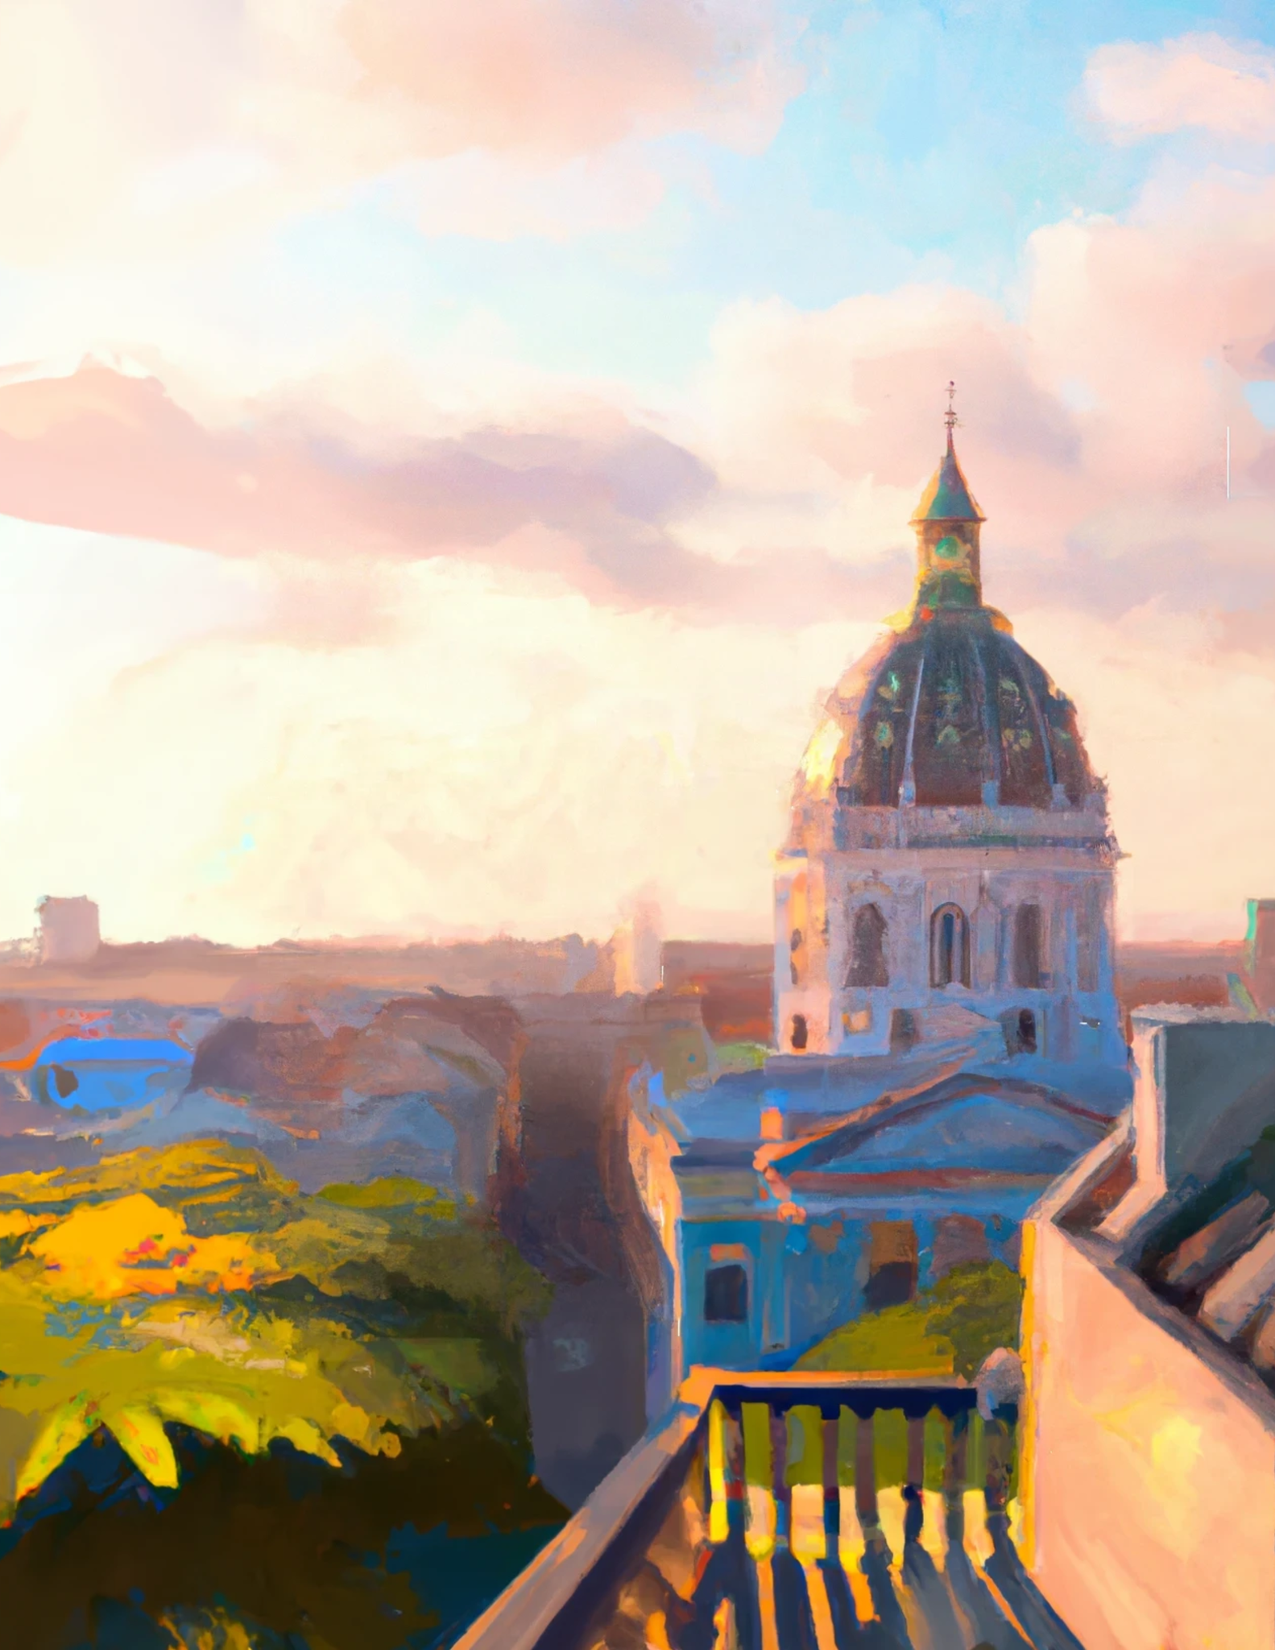
\includegraphics[width=\paperwidth,height=\paperwidth,keepaspectratio]{pictures/background.png}}}

    \begin{titlepage}
        \centering
        \vspace*{\fill}    
        \BgThispage
        {\huge\textsf{实\ 验\ 报\ 告}}\\[48pt]
        \reporttitle{实验名称}{Shell、Vim和数据整理}\\[72pt]
        \reportinfo{课程名称}{系统开发工具基础}\\[8pt]
        \reportinfo{学\hspace{\fill}号}{23070001092}\\[8pt]
        \reportinfo{学生姓名}{王佳晖}\\[8pt]
        \reportinfo{实验日期}{2024年8月30日}\\
        \href{https://github.com/JOINKINGER/TheSecondExperiment}{个人LaTex模版github链接}
        (https://github.com/JOINKINGER/TheSecondExperiment)
        \vspace*{\fill}
    \end{titlepage}

    \tableofcontents
    \newpage

    \NoBgThispage
    \section{实验目的}
    \begin{enumerate}    
        \item 学习Shell常见命令及使用方法
        \item 学习Vim的相关操作
        \item 学习正则表达式来处理数据
    \end{enumerate}
    
    \section{实验内容}
    \subsection{在/tmp下新建一个名为missing的文件夹。}
    \begin{enumerate}
        \item \textcolor{blue}{cd命令:用于在控制台中切换当前工作目录}\\
        \item \textcolor{blue}{ls命令:查看当前工作目录下的所有文件信息}\\[8pt]
        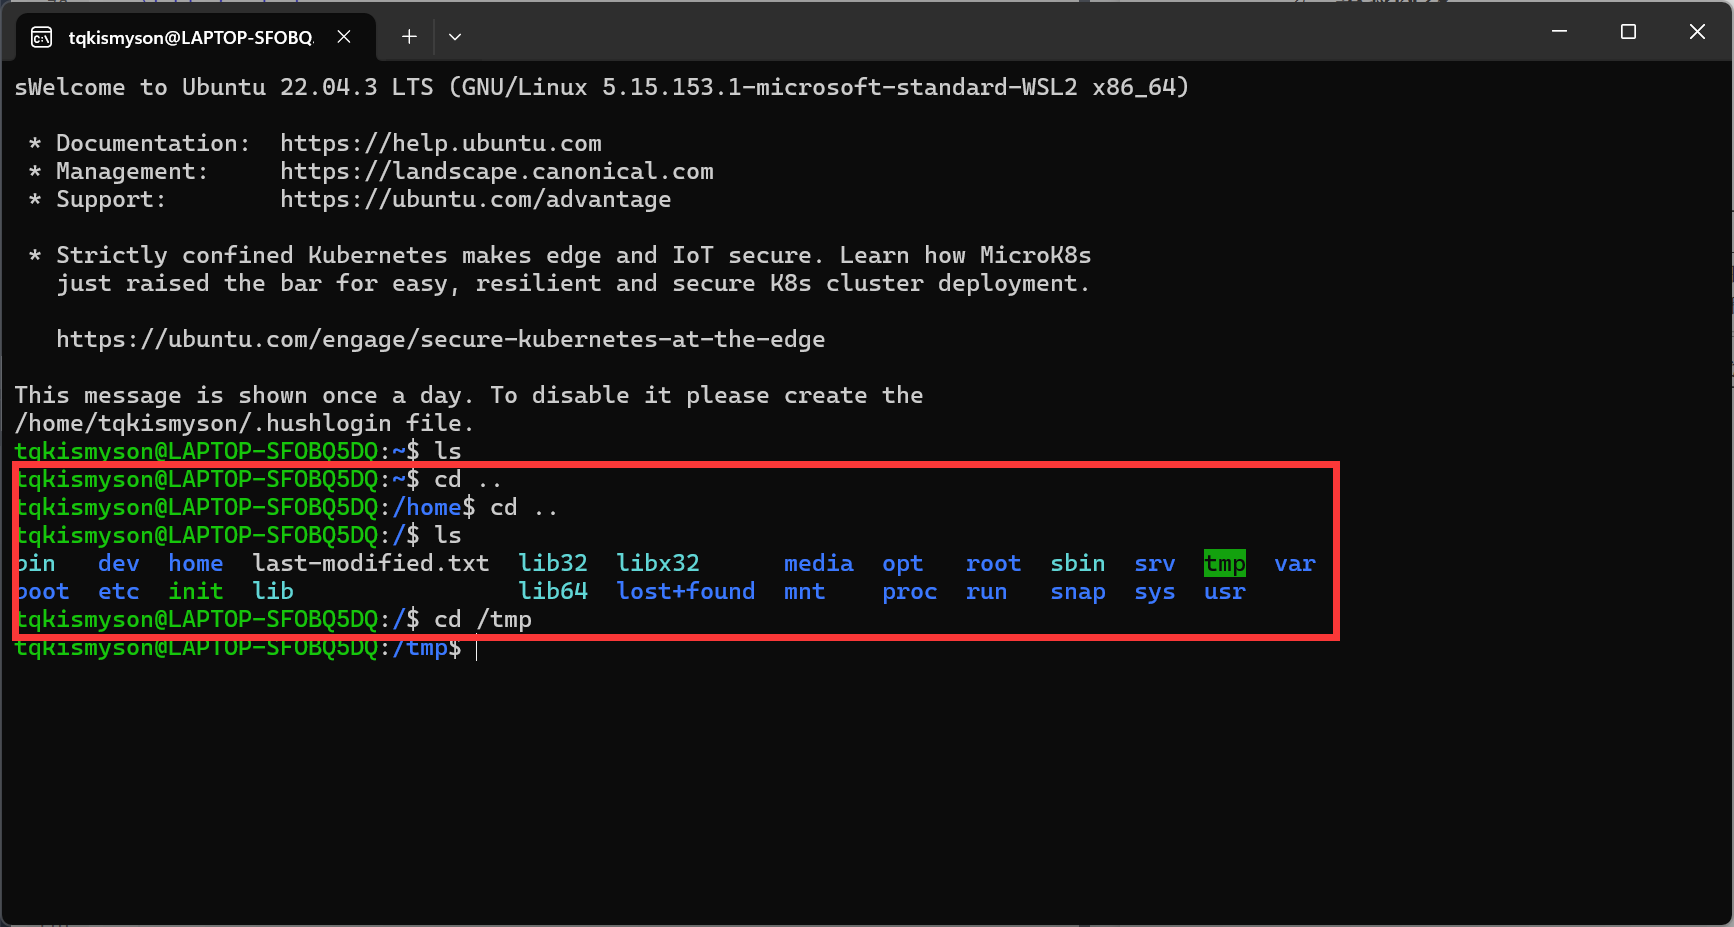
\includegraphics[scale=0.25]{pictures/Shell/1_1.png}
        首先cd..返回根目录\\
        接着ls查看文件信息\\
        最后cd到tmp文件夹中
        \item \textcolor{blue}{mkdir命令:在当前工作目录创建文件夹}\\[8pt]
        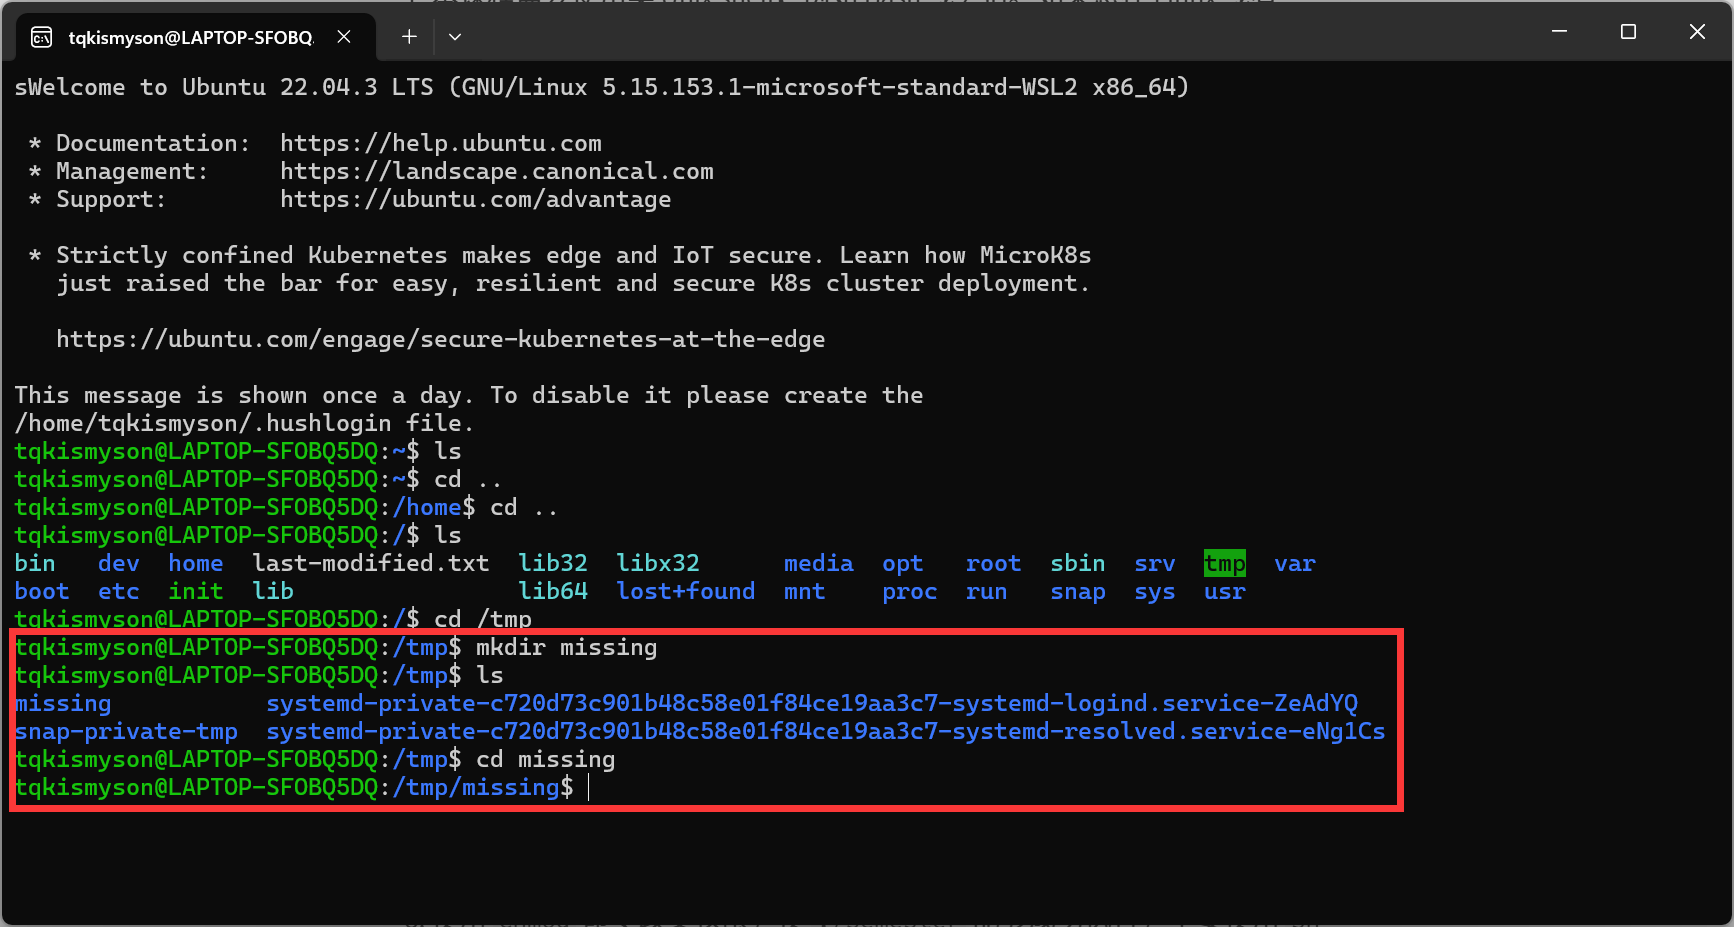
\includegraphics[scale=0.25]{pictures/Shell/1_2.png}
        mkdir创建missing文件夹\\
        ls查看是否创建成功\\
        cd到missing文件夹中\\
    \end{enumerate}
    \subsection{用touch在missing文件夹中新建一个叫semester的文件。}
    \begin{enumerate}
        \item \textcolor{blue}{man命令:查看用户手册}\\[8pt]
        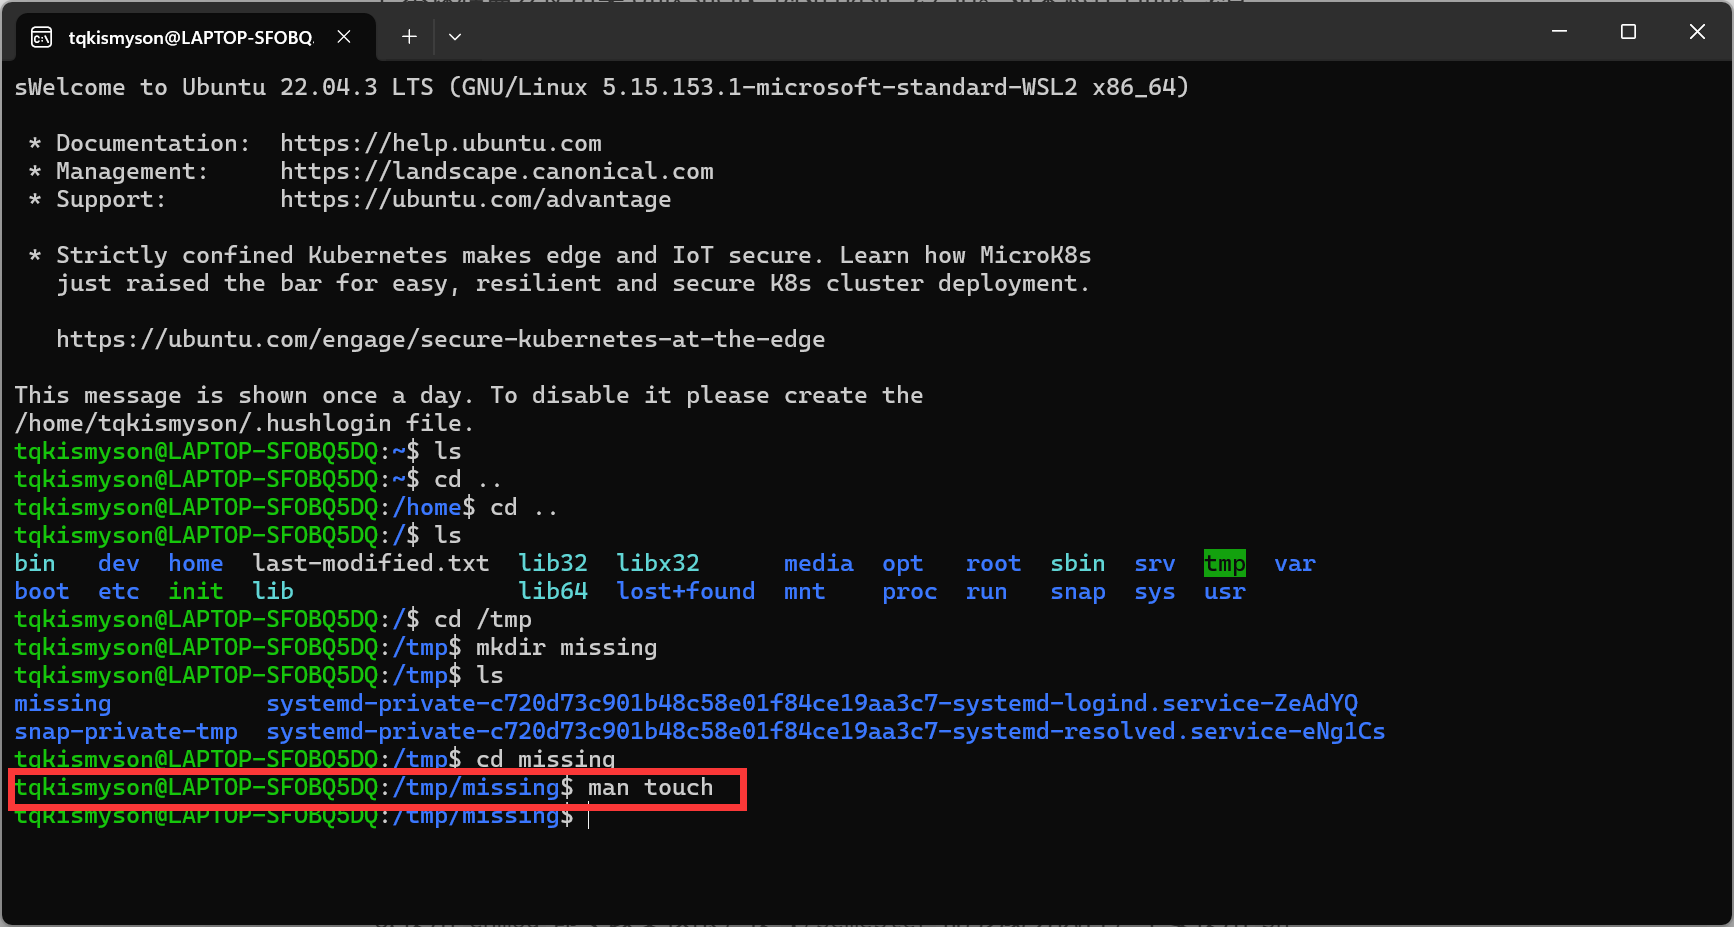
\includegraphics[scale=0.25]{pictures/Shell/2_1.png}  
        man查看touch的用法\\[8pt]
        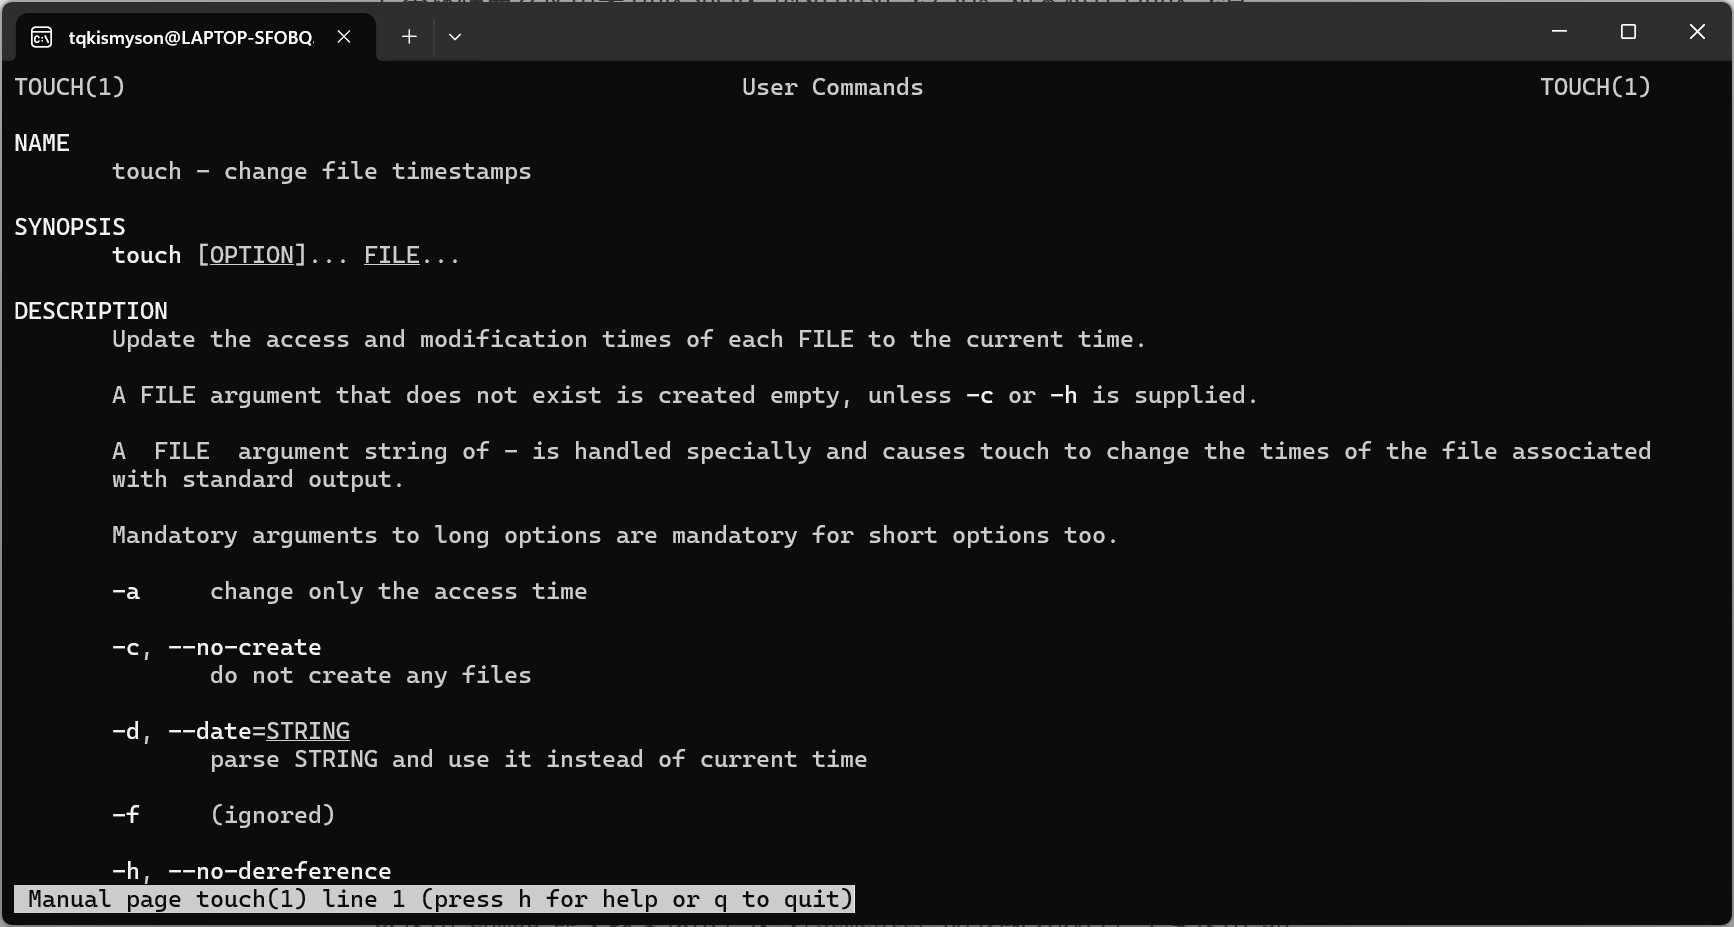
\includegraphics[scale=0.25]{pictures/Shell/2_2.png}
        \item \textcolor{blue}{touch命令:用于修改文件或者目录的时间属性,包括存取时间和更改时间。没有则新建}\\[8pt]
        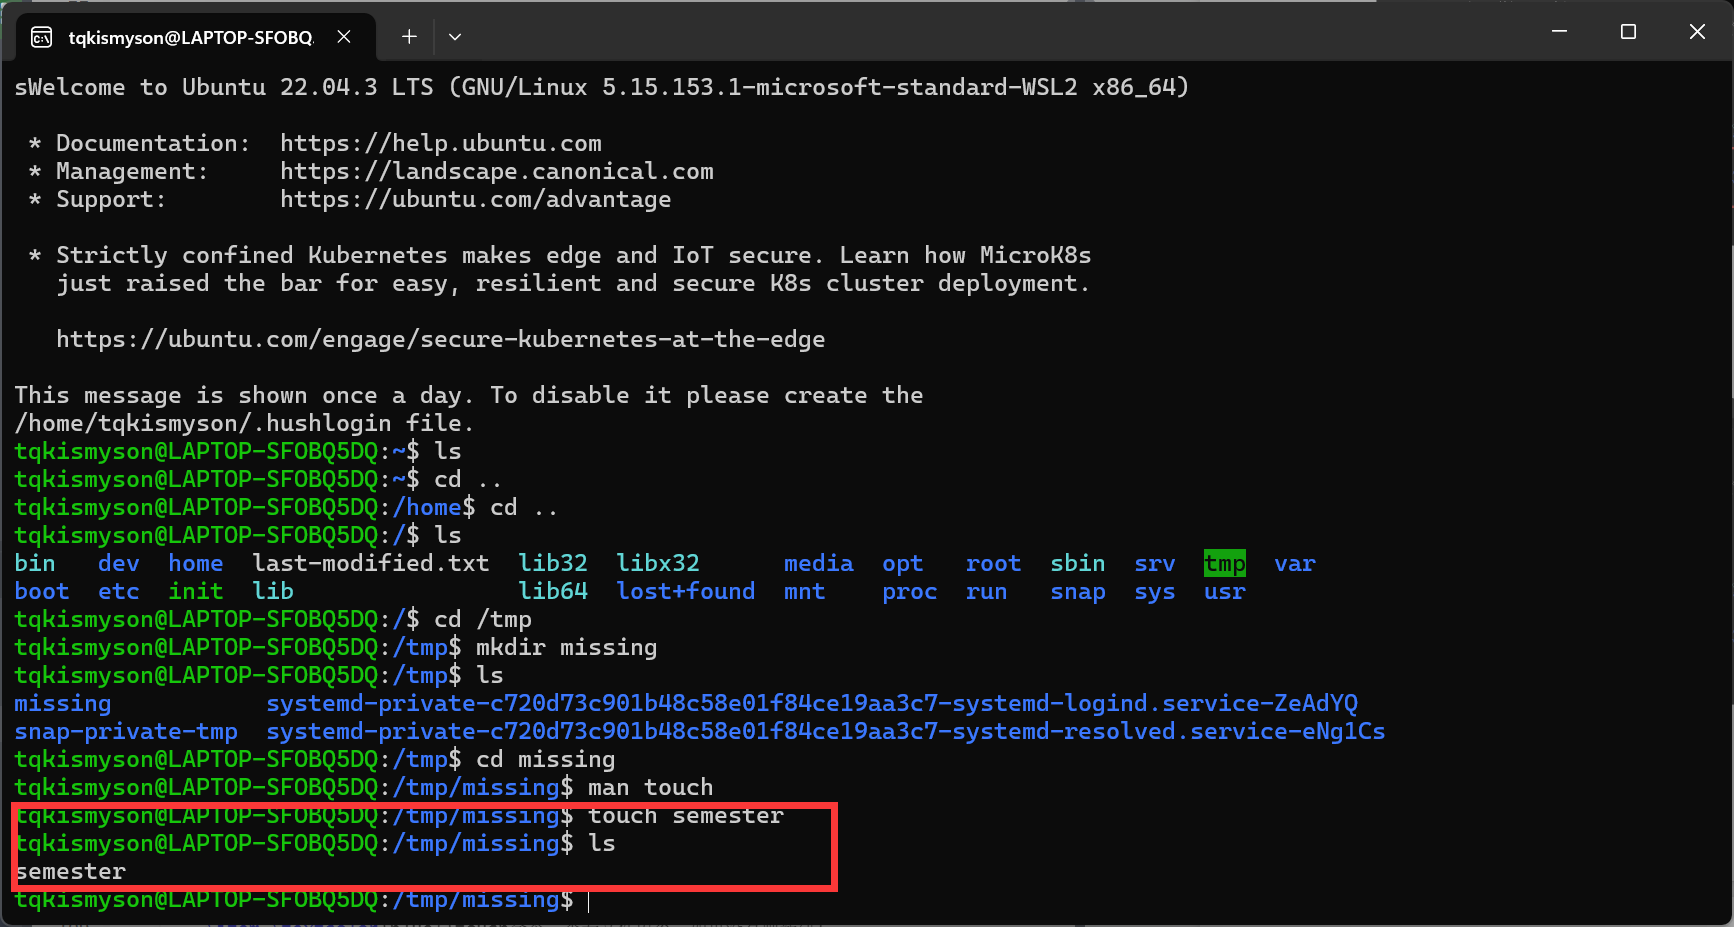
\includegraphics[scale=0.25]{pictures/Shell/2_3.png}
        touch新建semester文件(因为没有semester所以相当于新建)
    \end{enumerate}
    \subsection{将以下内容一行一行地写入semester文件。(文本内容略)}
    \begin{enumerate}
        \item \textcolor{blue}{echo命令:向控制台发送消息}\\
        \item \textcolor{blue}{echo >命令:向文件中覆写内容}\\
        \item \textcolor{blue}{echo > >命令:向文件追加写入内容}\\
        \item \textcolor{blue}{cat命令:查看文件内容}\\[8pt]
        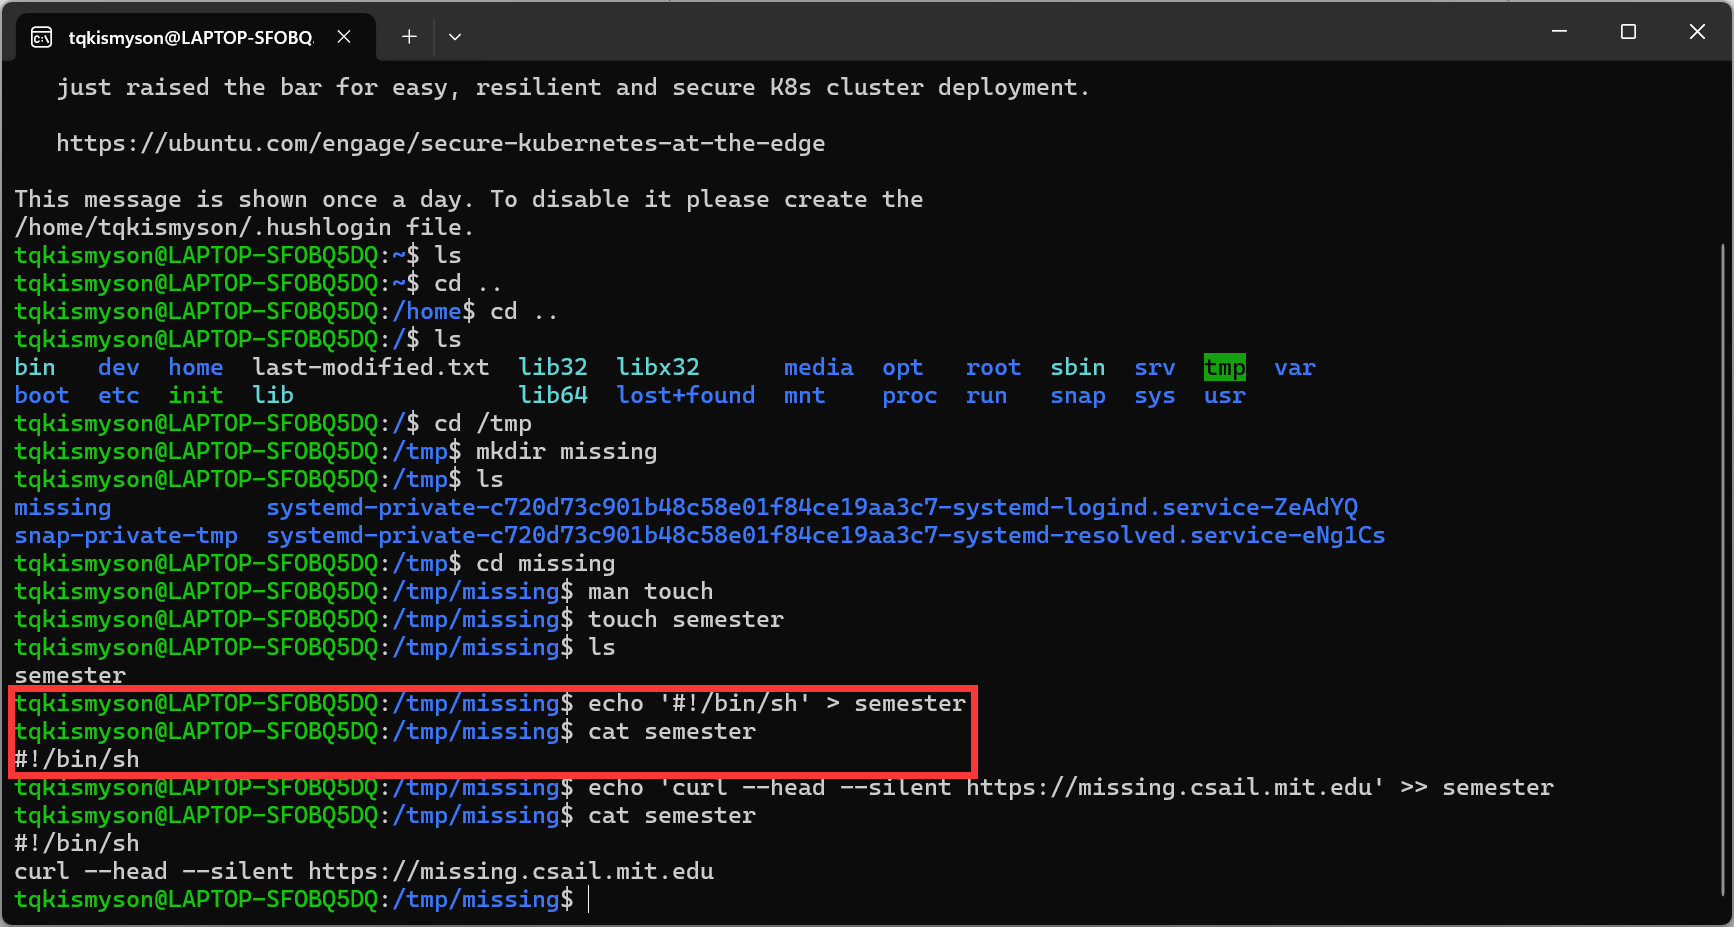
\includegraphics[scale=0.25]{pictures/Shell/3_1.png} 
        echo>向文件写入第一行内容\\
        cat查看文件内容\\[8pt]
        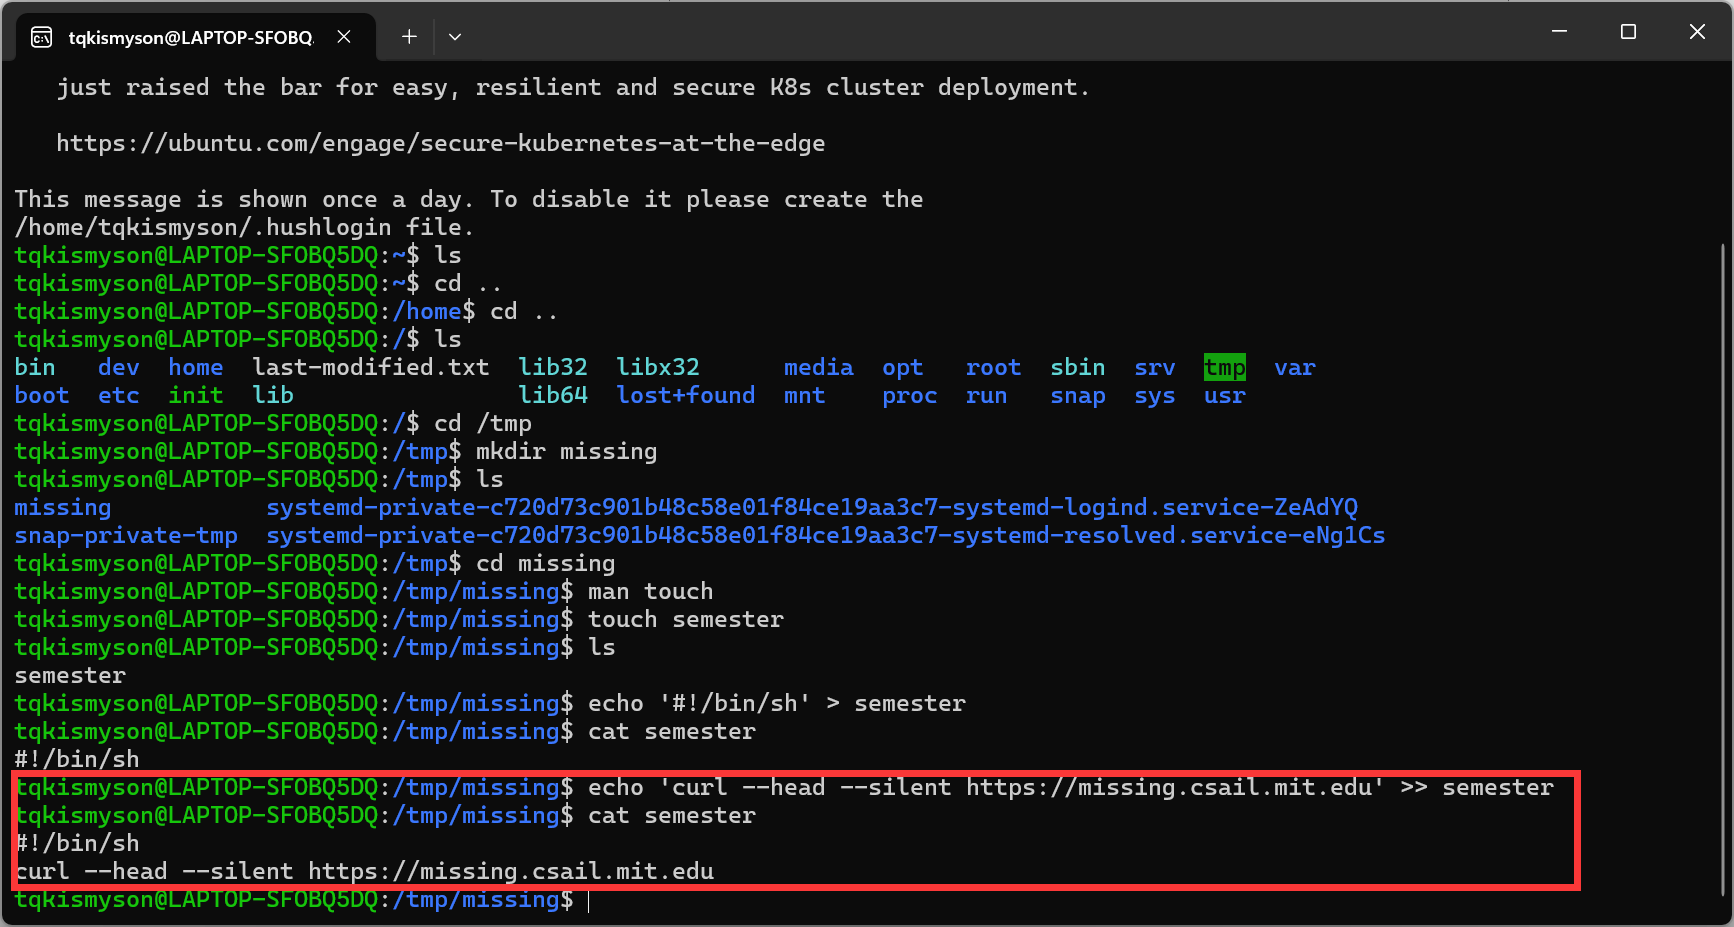
\includegraphics[scale=0.25]{pictures/Shell/3_2.png}
        echo>>向文件写入第二行内容\\
        cat再次查看是否写入成功\\
        \textcolor{red}{注:单引号可以使得转义符等直接以文本形式写入而不转义}
    \end{enumerate}
    \subsection{尝试执行semester文件}
    \begin{enumerate}
        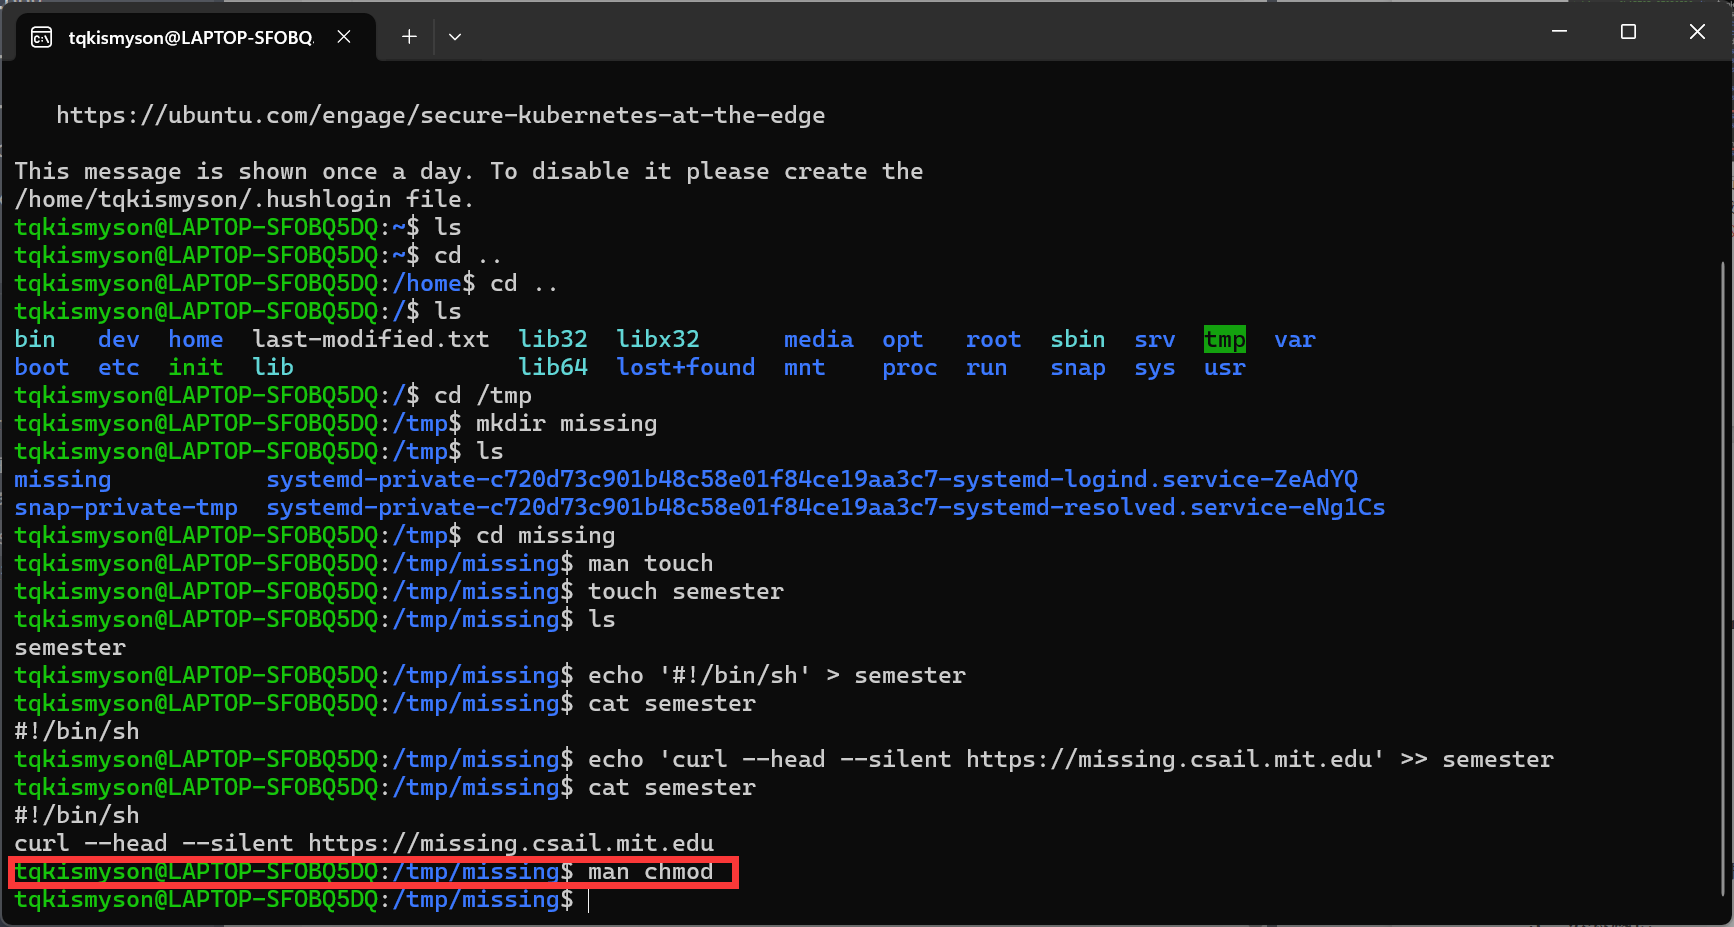
\includegraphics[scale=0.25]{pictures/Shell/4_1.png}
        man查看chmod使用说明\\[8pt]
        \item \textcolor{blue}{1.chmod命令:添加权限}\\[8pt]
        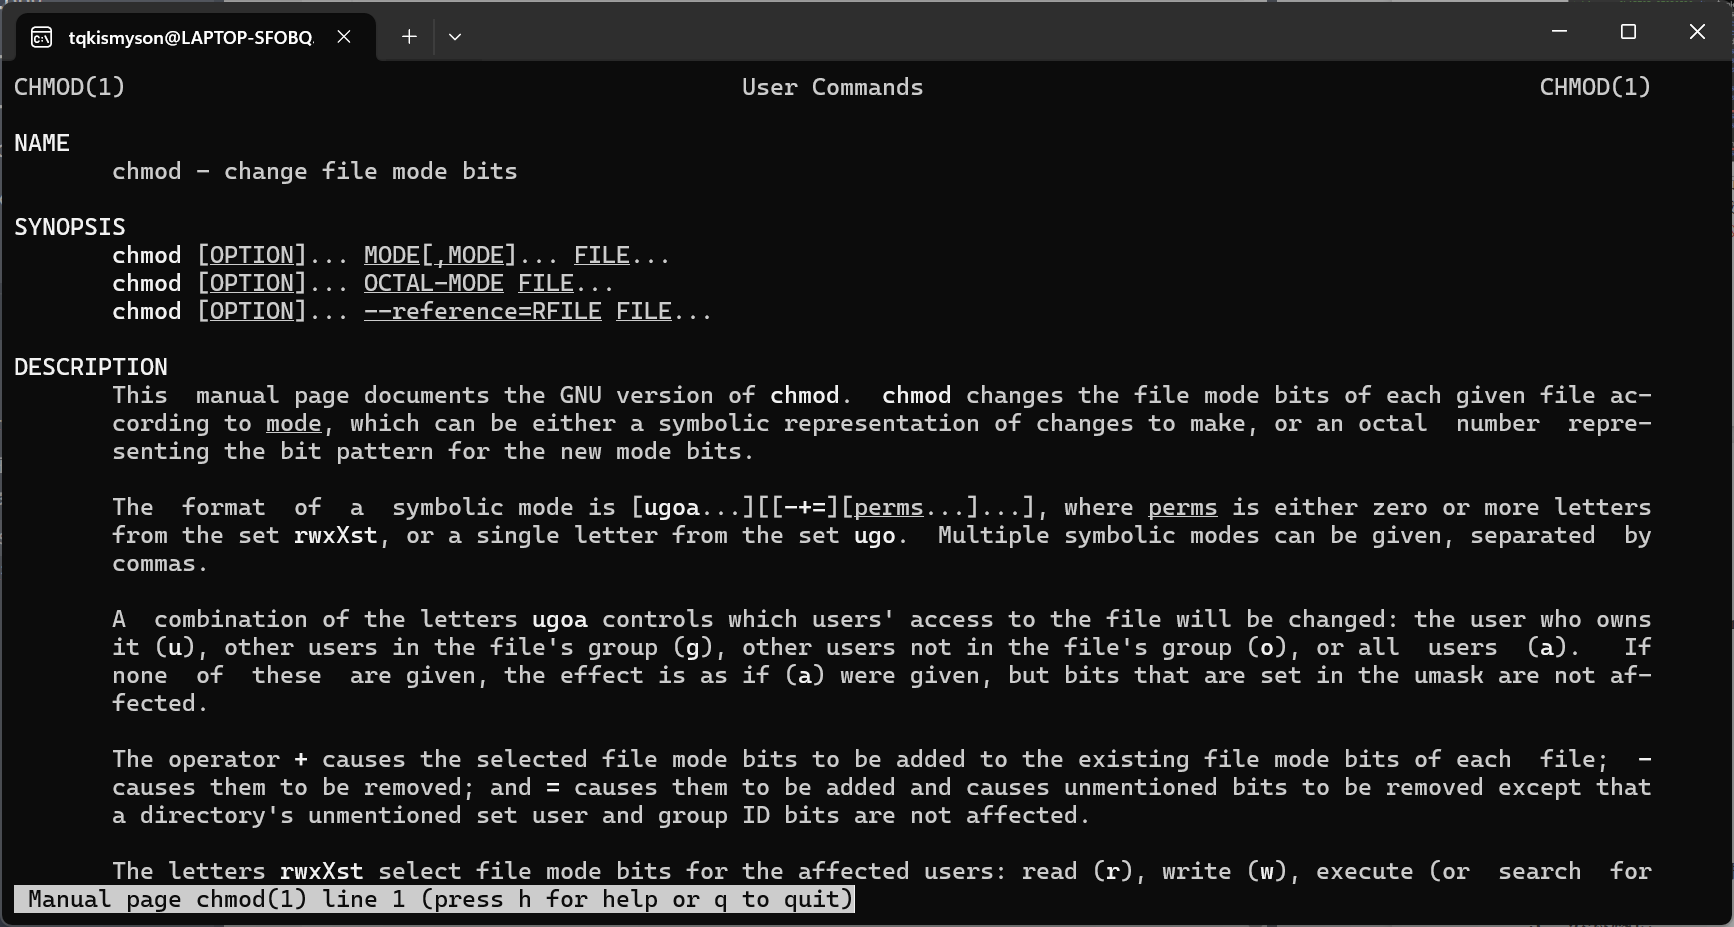
\includegraphics[scale=0.25]{pictures/Shell/4_2.png}  
        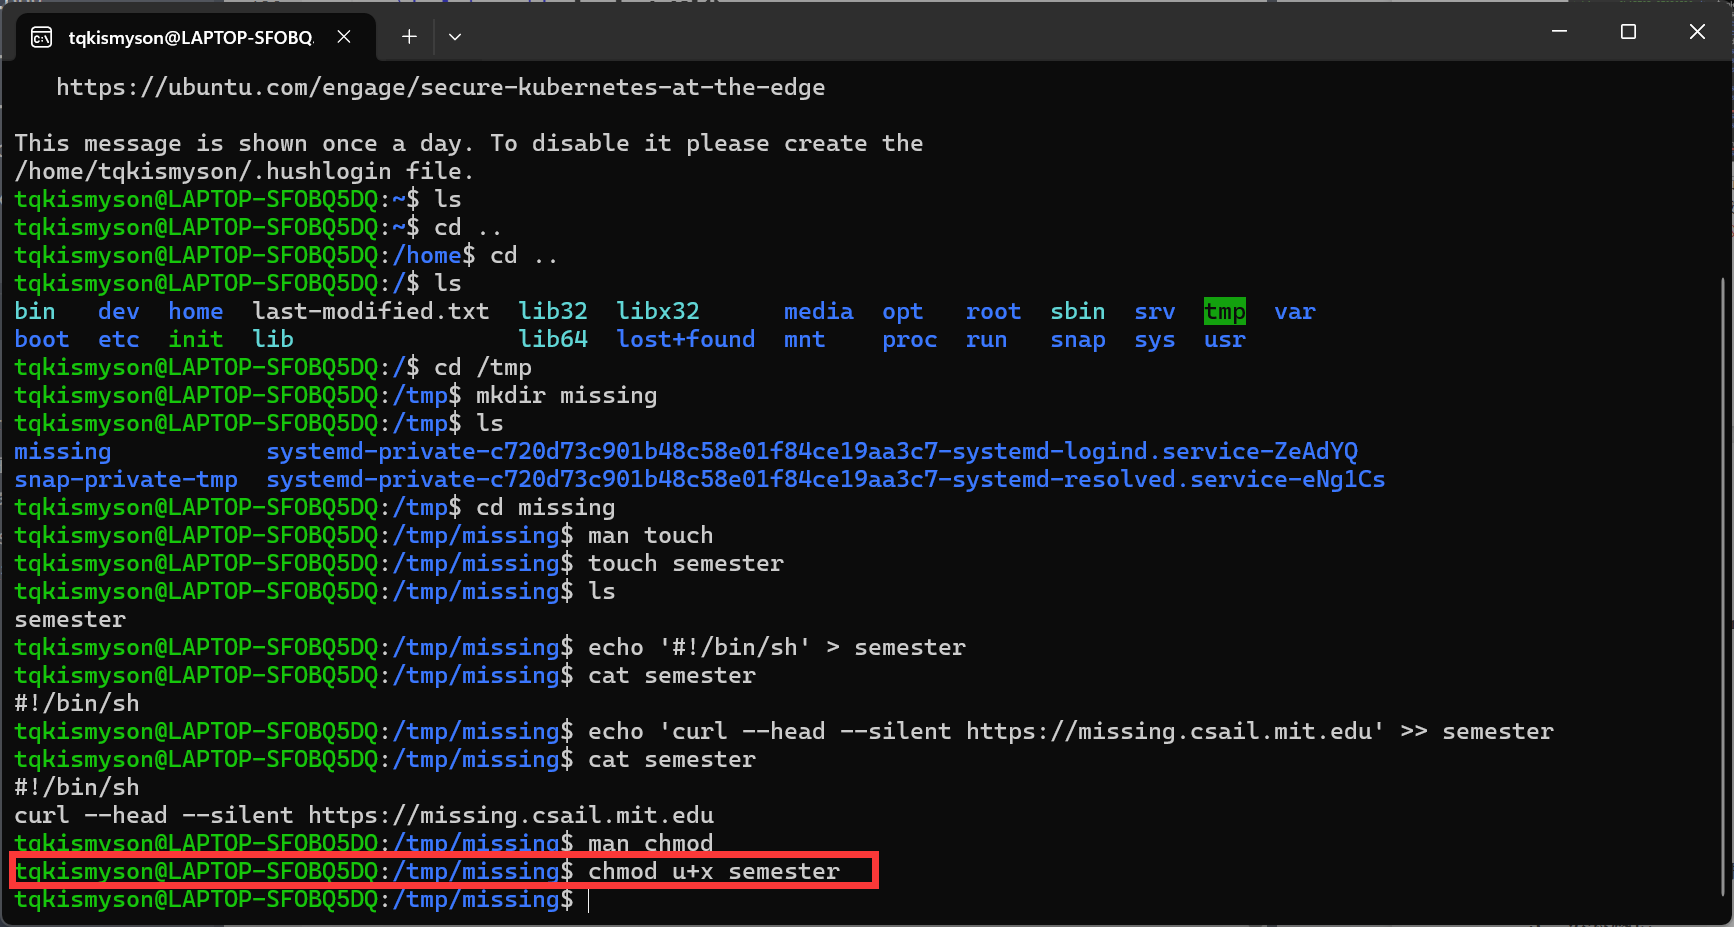
\includegraphics[scale=0.25]{pictures/Shell/4_3.png} 
        chmod a+x给全体用户添加执行权限\\[6pt]
        \textcolor{red}{注:x表示执行权限}\\
        \item \textcolor{blue}{2./命令:运行可执行文件}
        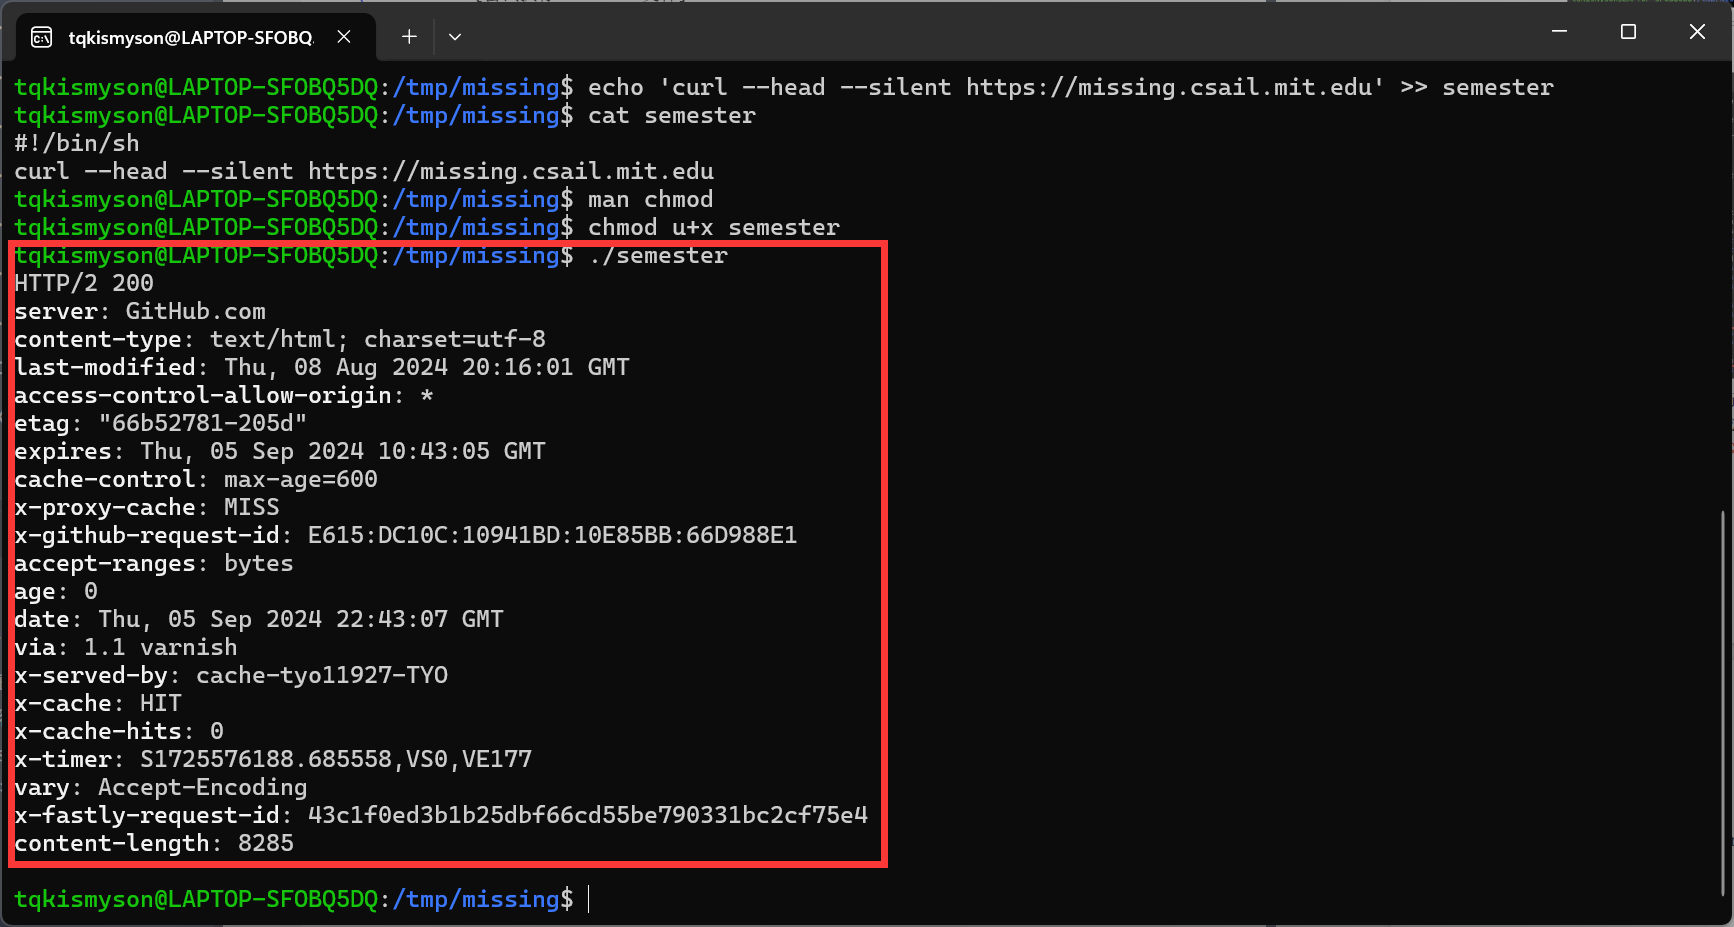
\includegraphics[scale=0.25]{pictures/Shell/4_4.png} 
        ./运行semester文件\\[8pt]
    \end{enumerate}
    \subsection{使用ls完成如下操作(操作见网站)}
    \begin{enumerate}
        \item \textcolor{blue}{-l(长列表格式)显示文件的详细信息}\\
        \item \textcolor{blue}{-a 显示所有文件,包括以点(.)开头的隐藏文件}\\
        \item \textcolor{blue}{-h 以人类可读的格式显示文件大小}\\
        \item \textcolor{blue}{--color=auto 确保输出以彩色显示,这在大多数现代终端中是默认行为,但明确指定可以避免在某些环境下的问题}\\[8pt]
        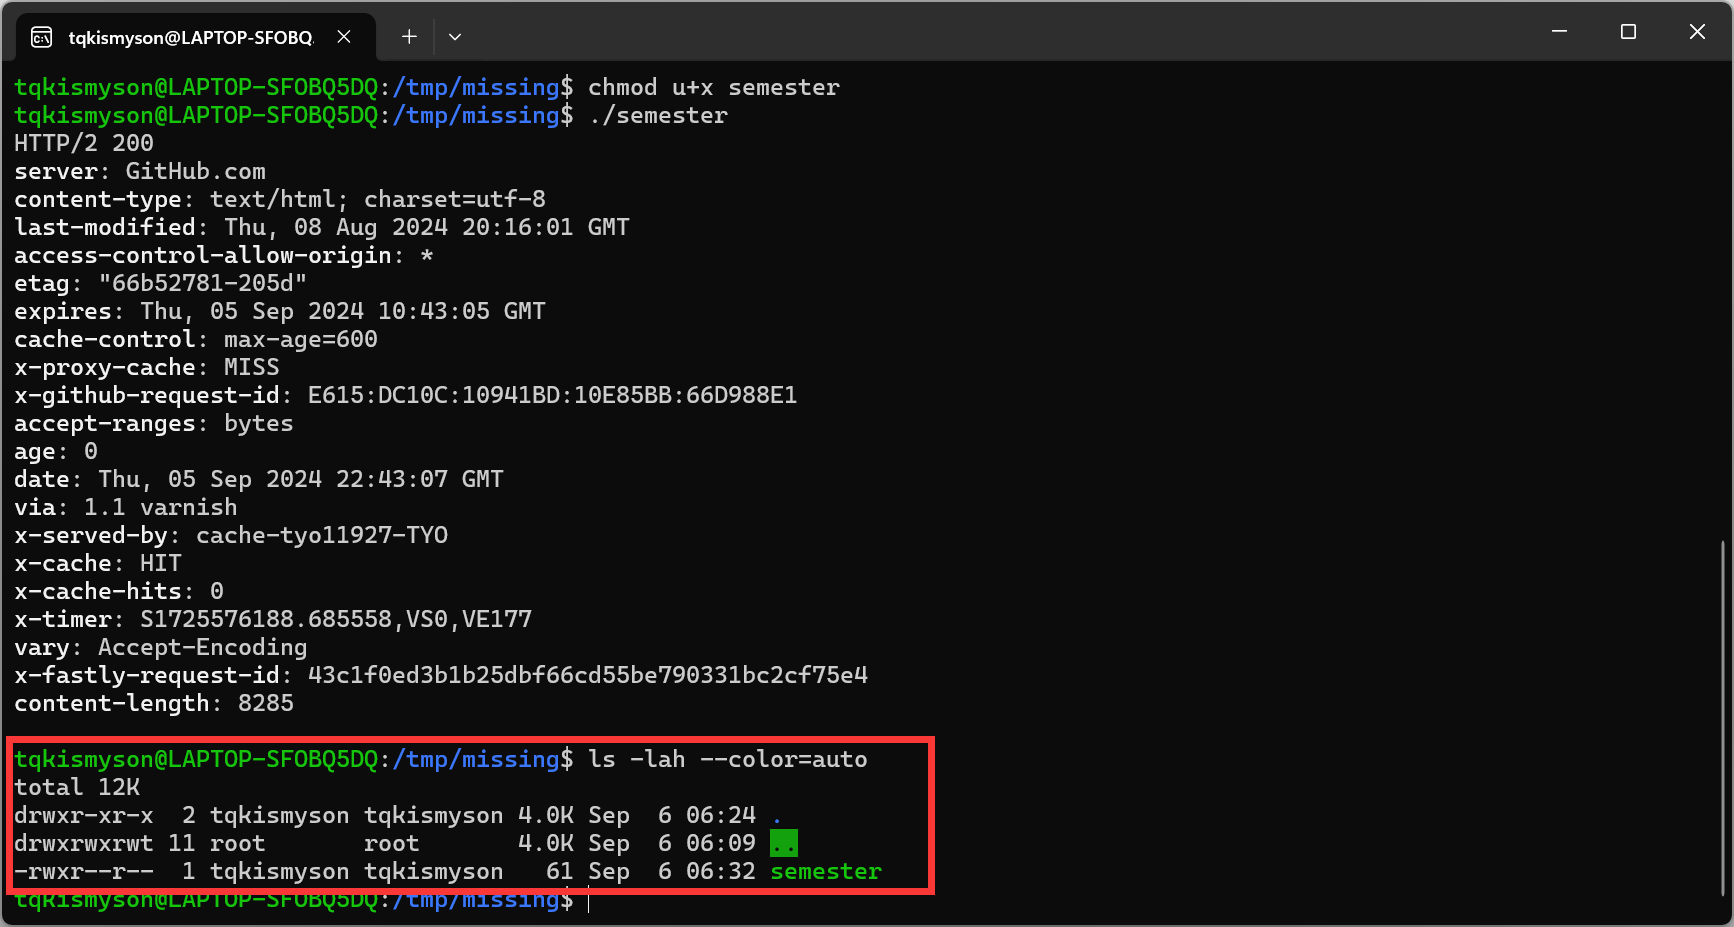
\includegraphics[scale=0.25]{pictures/Shell/5_1.png}  
    \end{enumerate}
    \subsection{编写两个bash函数marco和polo执行下面的操作(操作见网站)}
    \begin{enumerate}
        \item \textcolor{blue}{vim命令:通过vim编辑文件}\\[8pt]
        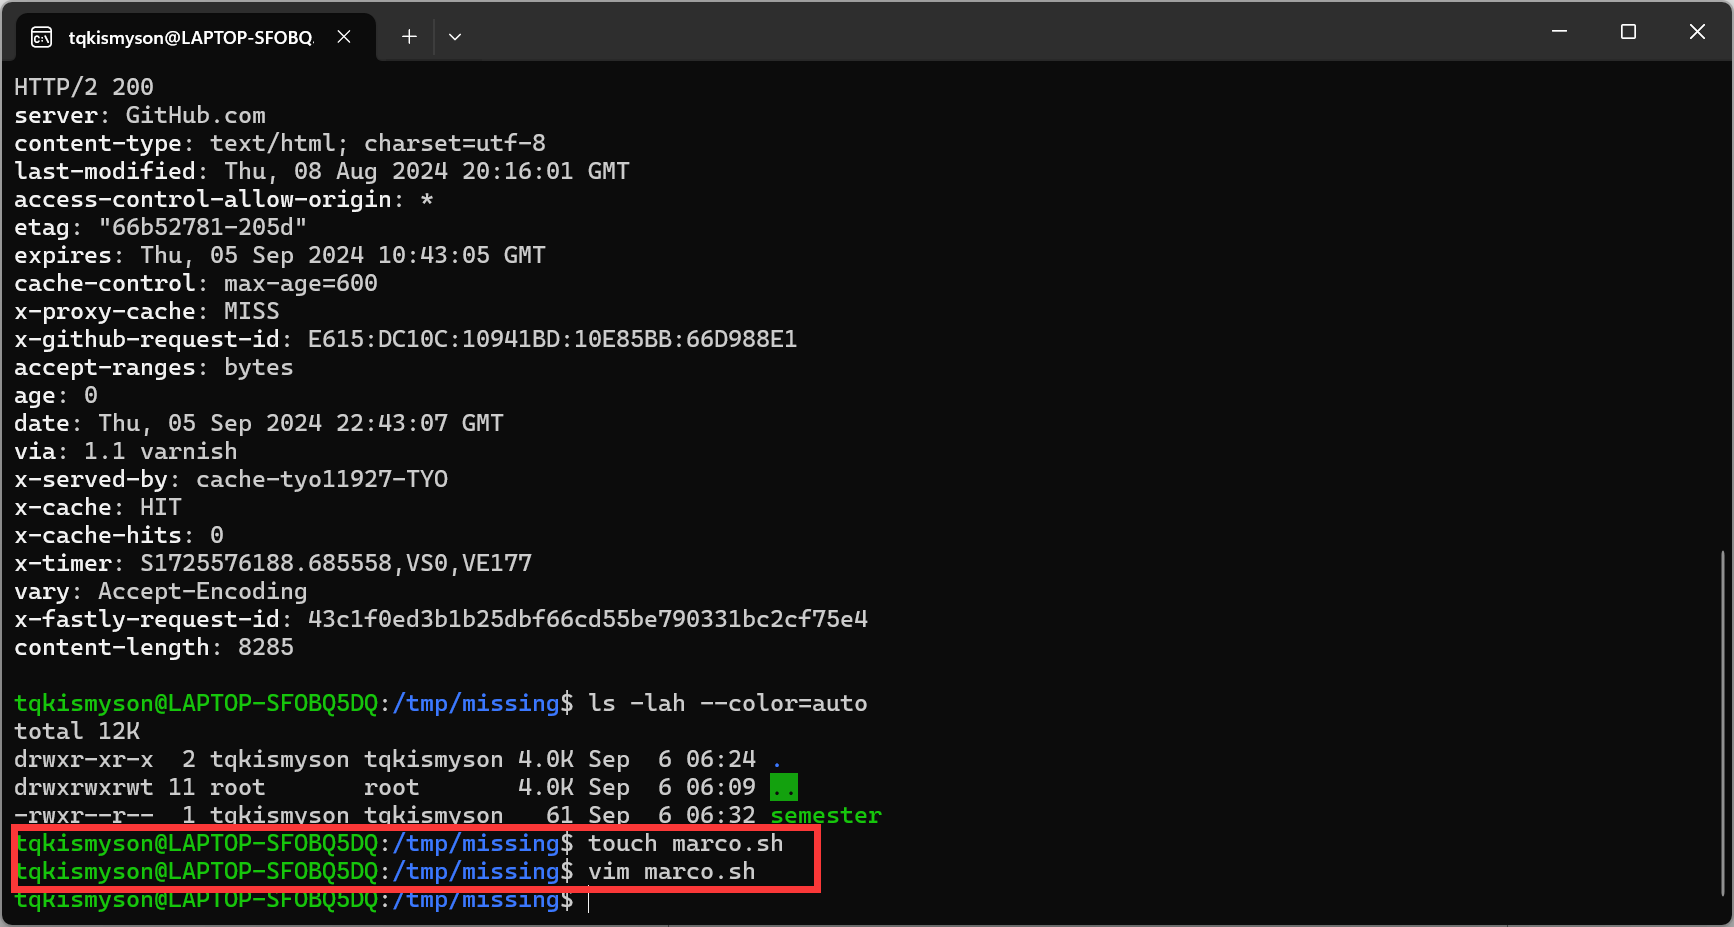
\includegraphics[scale=0.25]{pictures/Shell/6_1.png}  
        touch创建marco.sh文件\\
        vim打开该文件\\[8pt]
        \item \textcolor{blue}{按I进入INSERT(编辑)模式}\\[8pt]
        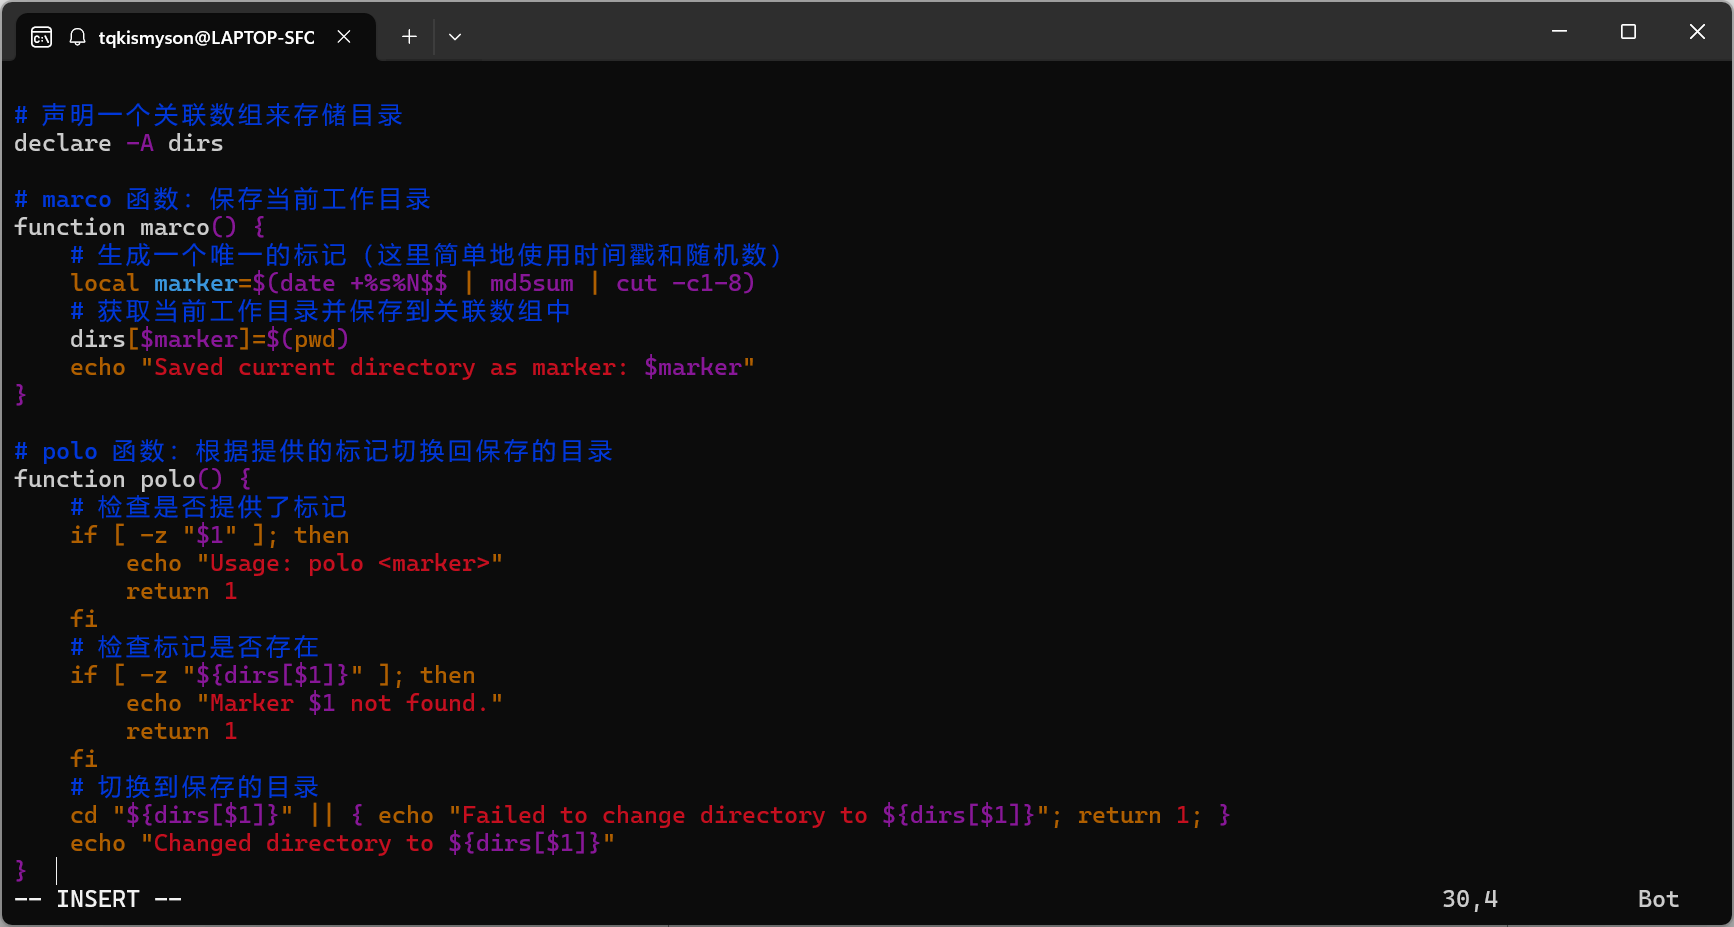
\includegraphics[scale=0.25]{pictures/Shell/6_2.png}\\
        输入代码\\[8pt]
        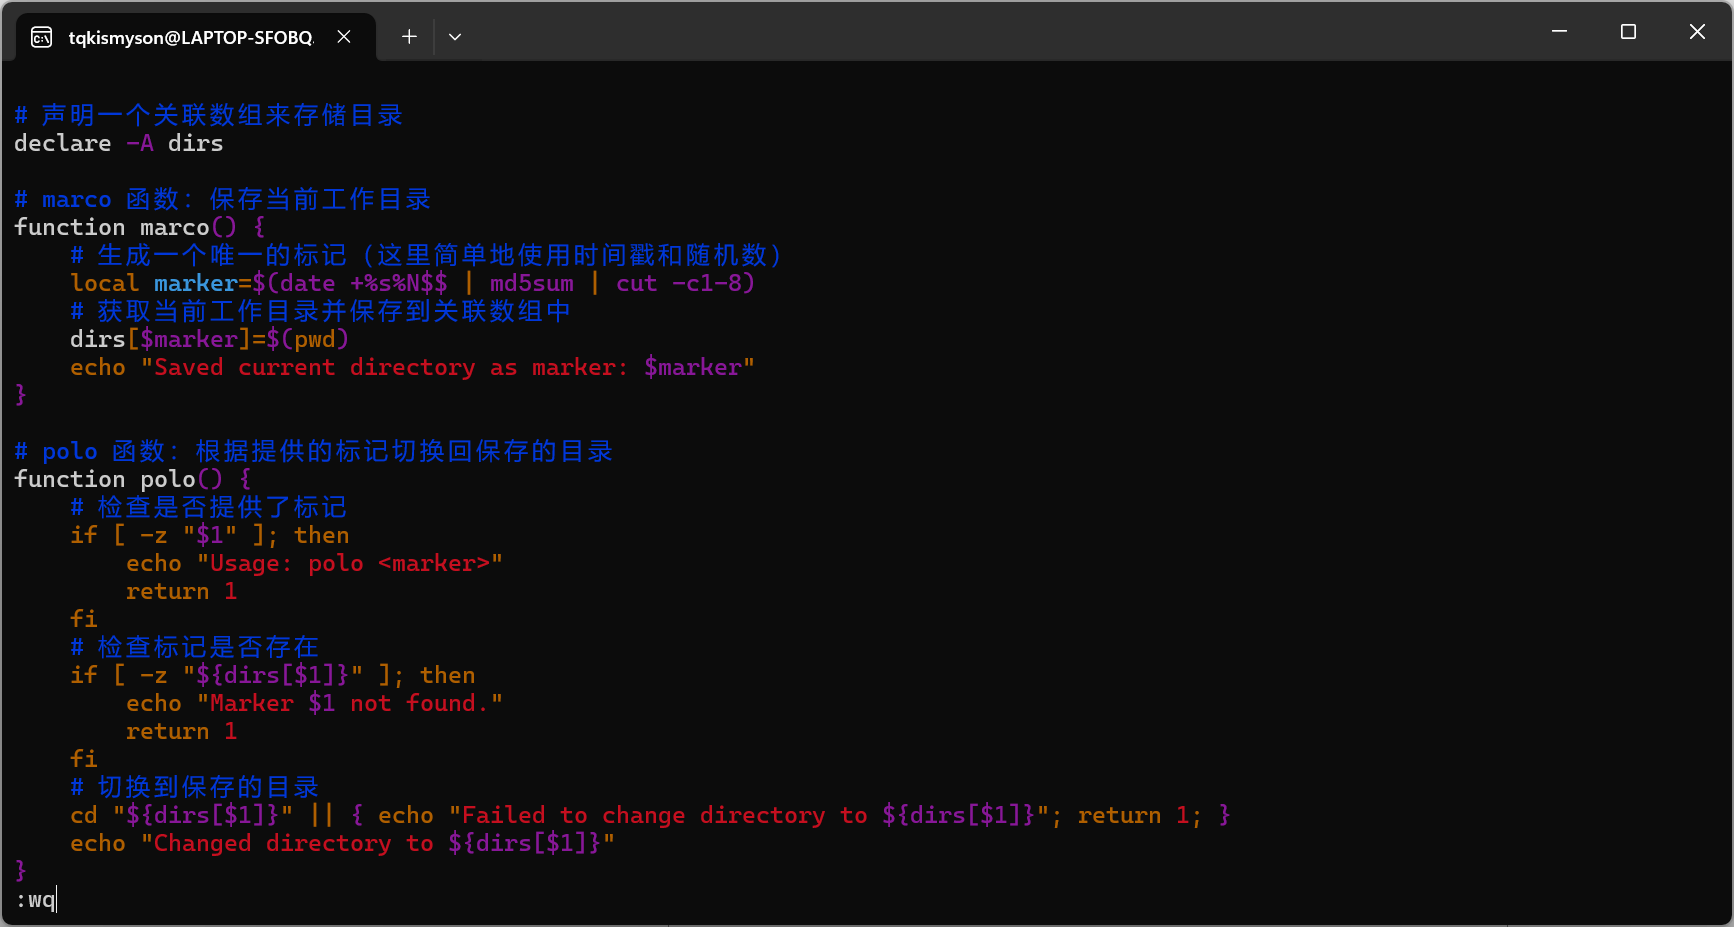
\includegraphics[scale=0.25]{pictures/Shell/6_3.png}
        按ESC退出编辑模式,输入:wq保存并退出\\
        \item \textcolor{blue}{source命令:加载函数}\\[8pt]
        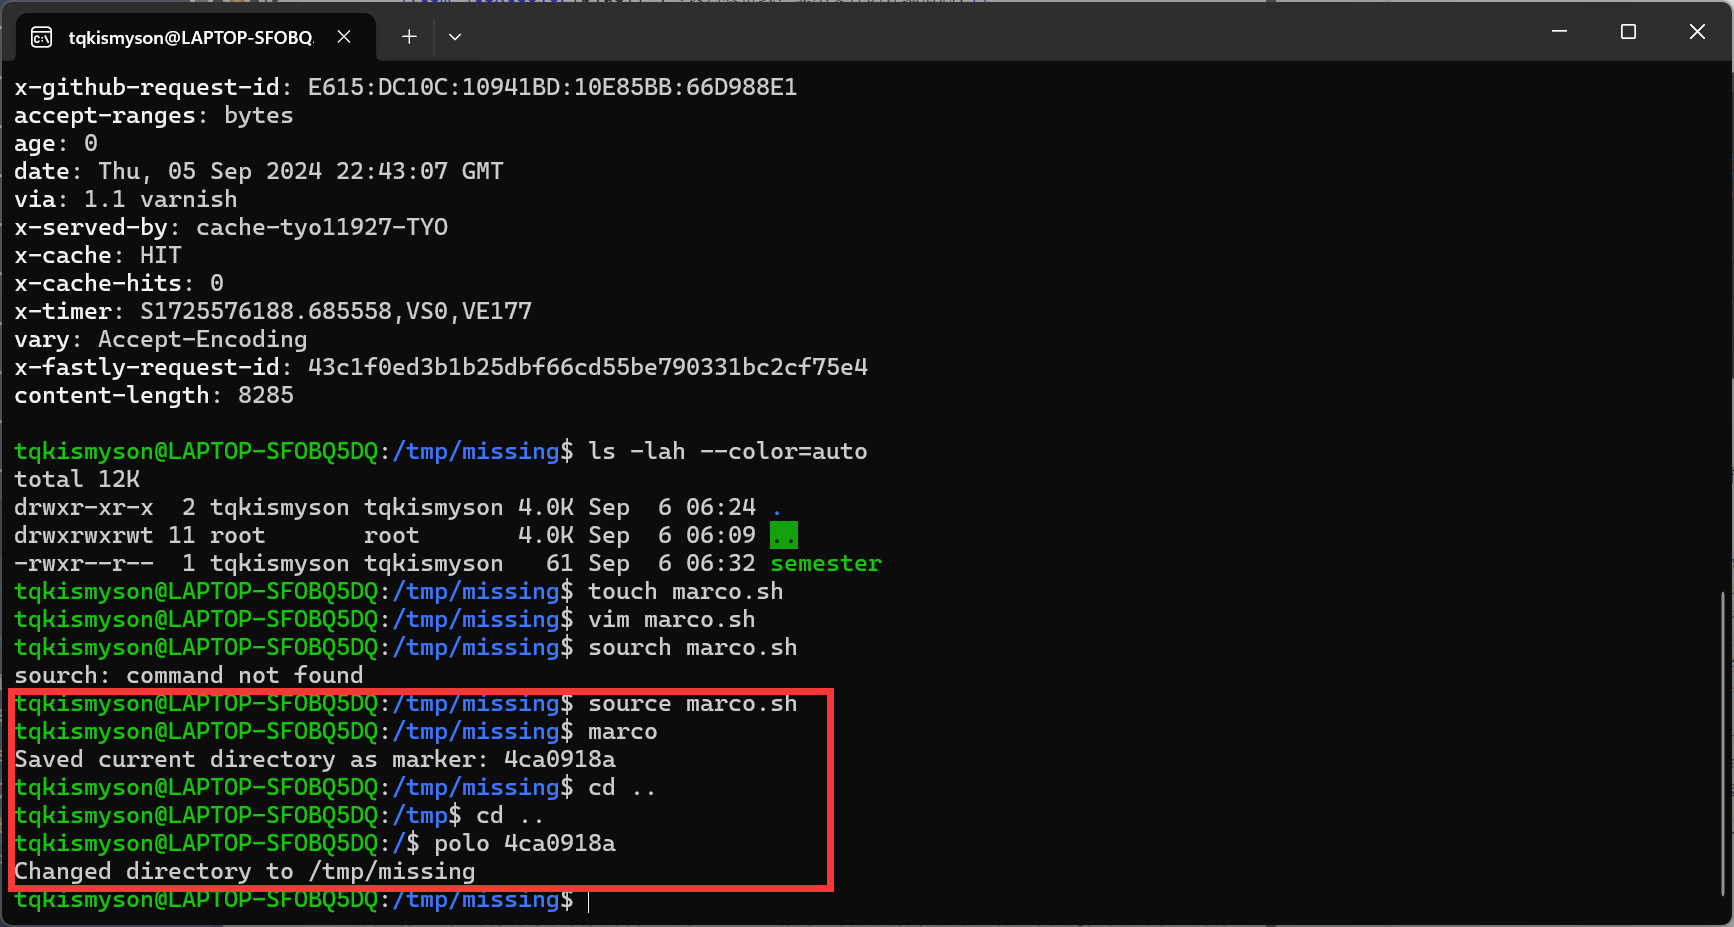
\includegraphics[scale=0.25]{pictures/Shell/6_4.png}
        source加载marco和polo函数\\
        marco记录当前文件夹\\
        cd..返回根目录\\
        polo返回记录文件夹\\
        发现函数运行成功
    \end{enumerate}

    \NoBgThispage
    \subsection{问题:进行原地替换听上去很有诱惑力,例如: sed s/REGEX/SUBSTITUTION/ input.txt > input.txt。但是这并不是一个明智的做法,为什么呢?还是说只有 sed 是这样的? 查看 man sed 来完成这个问题}
    \begin{enumerate}
        \item \textcolor{blue}{不是,因为有数据丢失的风险:}
        当使用 > 进行重定向时,如果 sed 命令执行失败或因为某些原因没有按预期工作,那么原文件 input.txt 的内容可能会被清空。这是因为 > 操作符会先清空目标文件,然后再将输出写入。如果 sed 在清空文件后遇到错误而未能成功写入新内容,那么文件就会保持为空状态,导致数据丢失。
        \item \textcolor{blue}{并非所有工具都如此:}\\
        虽然直接使用 > 重定向来修改原文件对于 sed 来说是不推荐的,但这并不意味着所有工具或命令都有这样的风险。一些工具提供了专门的选项或方法来安全地原地修改文件。例如,sed 本身就有 -i(in-place)选项,允许它直接修改文件内容而不是输出到标准输出。
        \item \textcolor{blue}{查看man sed后,得知sed的-i选项:}\\
        为了安全地在原地修改文件,你可以使用 sed 的 -i 选项。例如,sed -i 's/REGEX/SUBSTITUTION/' input.txt 会直接在 input.txt 文件中进行替换,不会输出到标准输出,也不会创建临时文件(除非你的 sed 版本要求)。注意,某些 sed 实现(如 GNU sed)允许你指定一个扩展名,用于在修改前创建原文件的备份,如 sed -i.bak 's/REGEX/SUBSTITUTION/' input.txt。
    \end{enumerate}
    \subsection{找出最近十次开机的开机时间平均数、中位数和最长时间。}
    \begin{enumerate}
        \item 
        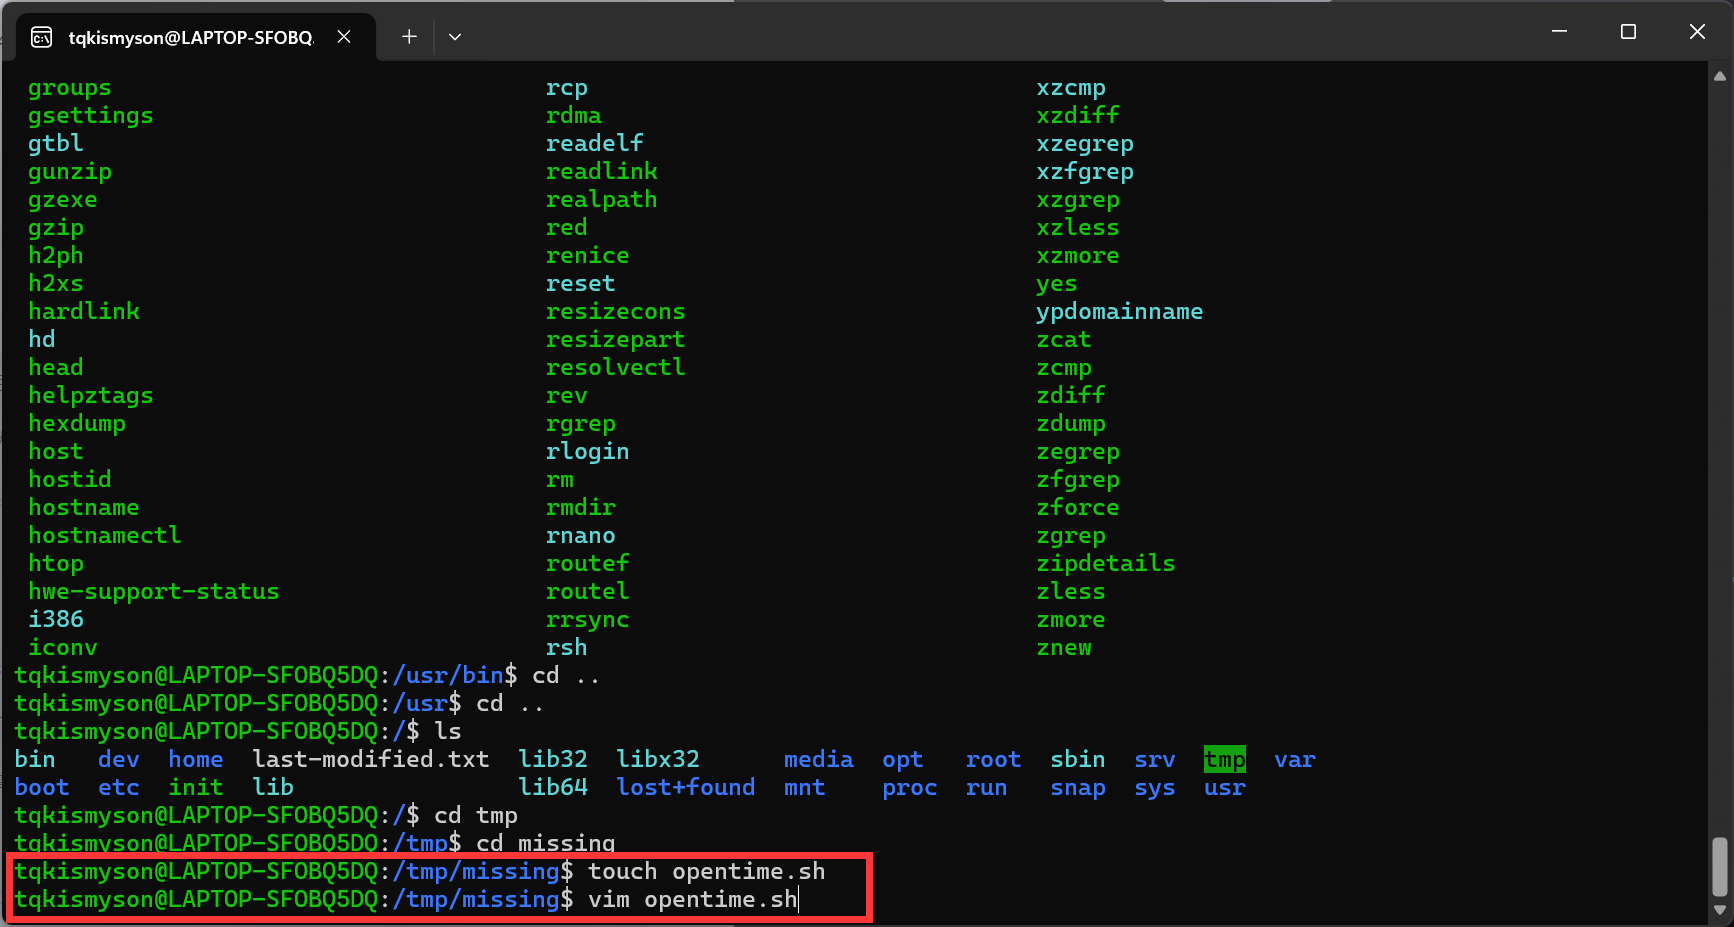
\includegraphics[scale=0.25]{pictures/Shell/7_1.png}
        \textcolor{blue}{touch新建opentime.sh的bash文件}\\
        \textcolor{blue}{vim打开该文件}\\[8pt]
        \item 
        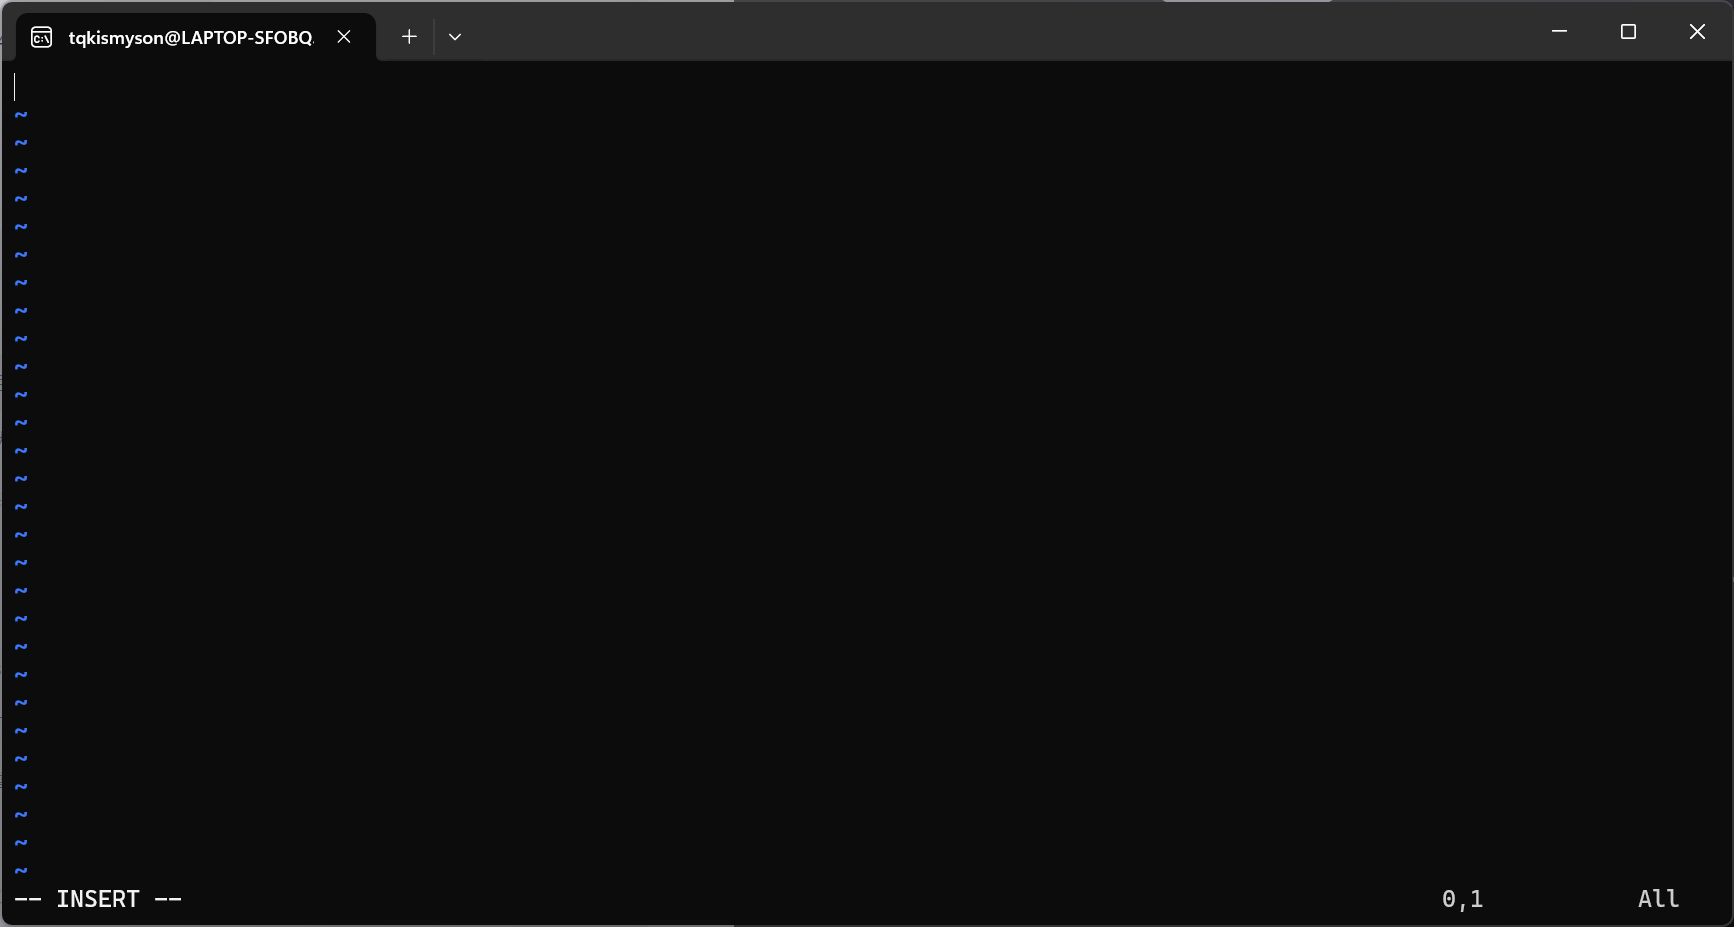
\includegraphics[scale=0.25]{pictures/Shell/7_2.png}
        \textcolor{blue}{按I进入INSERT(编辑)模式}\\[8pt]
        \item 
        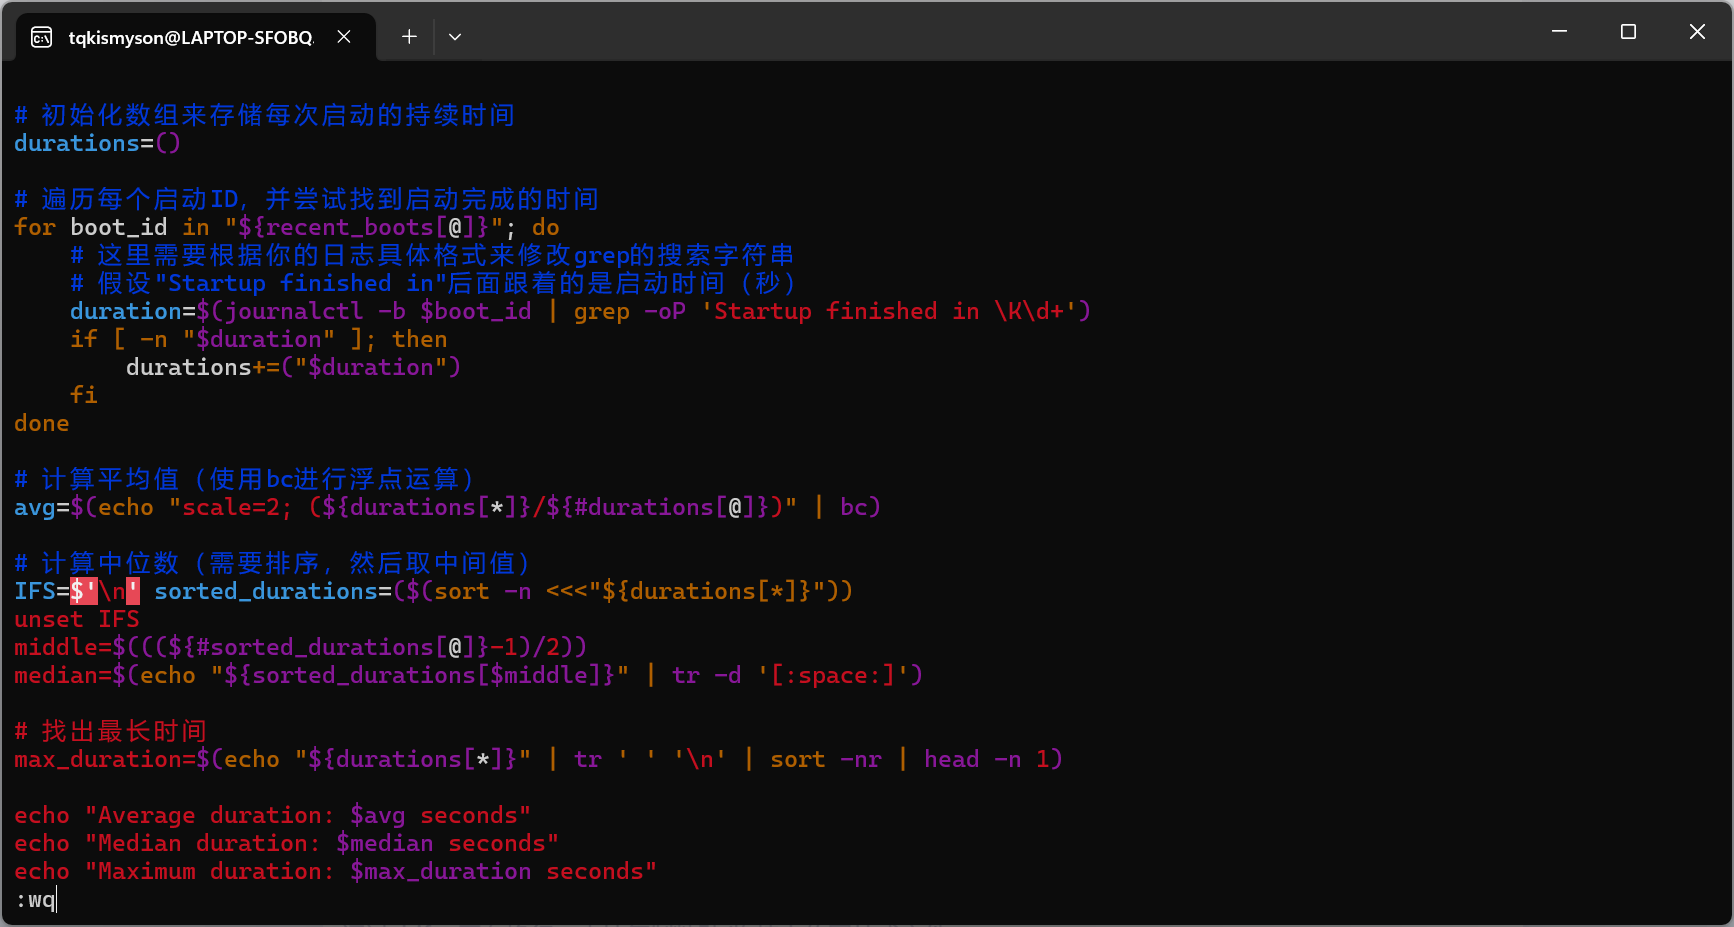
\includegraphics[scale=0.25]{pictures/Shell/7_3.png}
        \textcolor{blue}{编辑代码}\\
        \textcolor{blue}{按ESC后输入:wq保存并退出}\\[8pt]
        \item 
        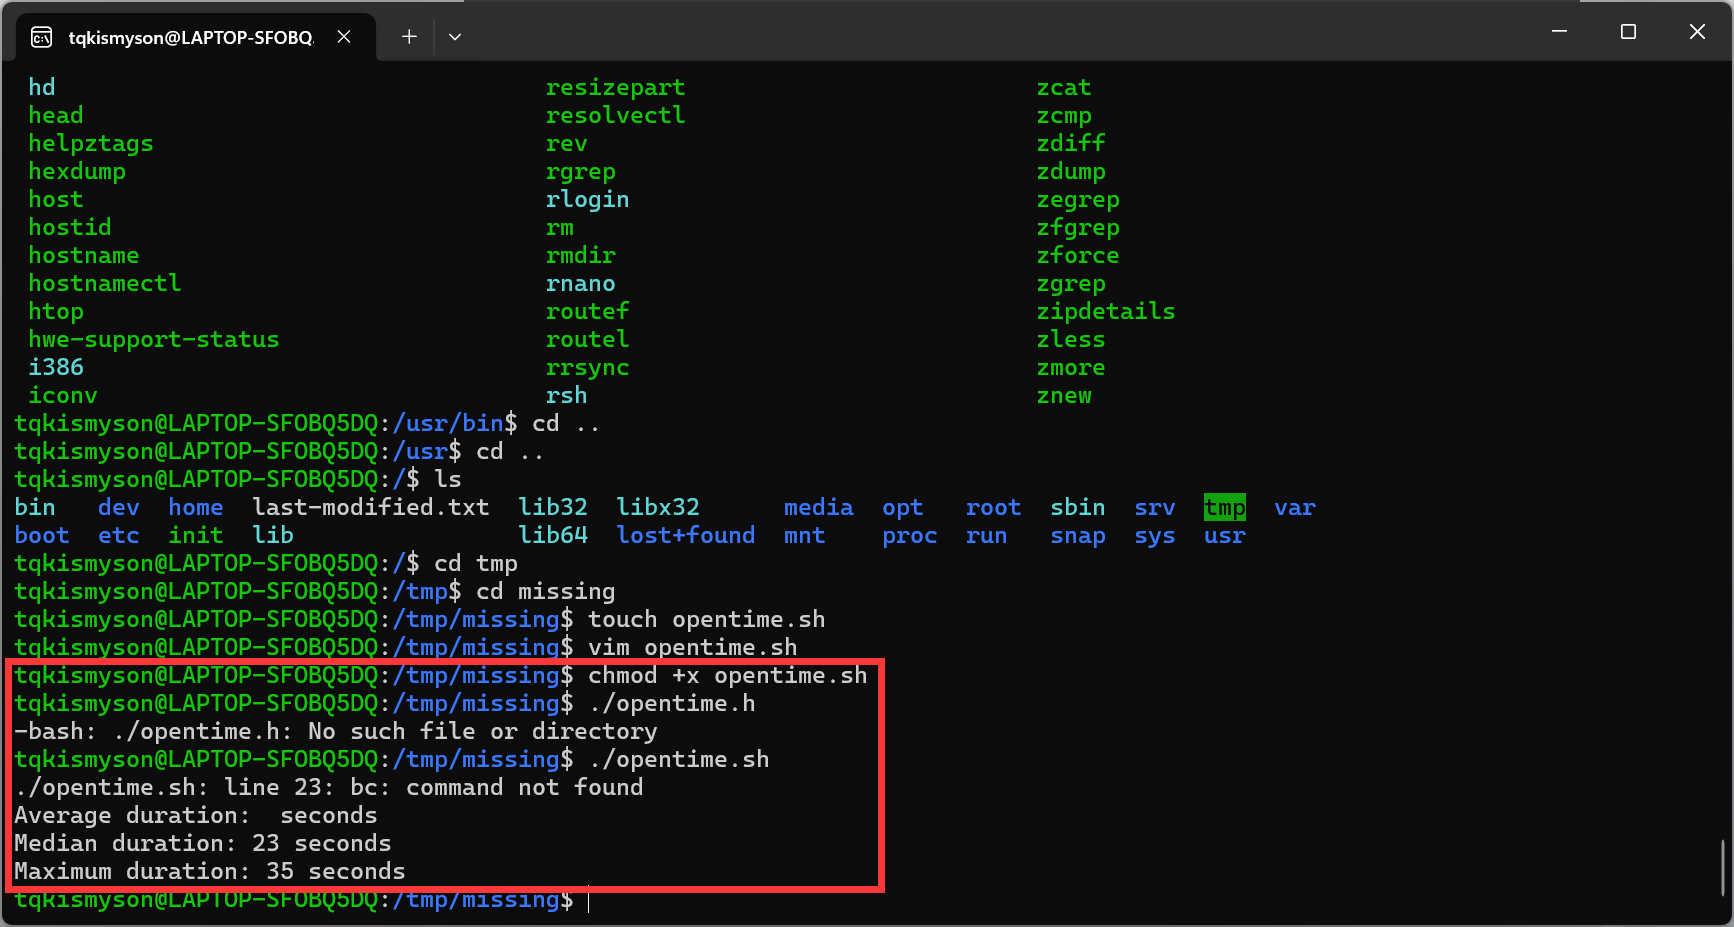
\includegraphics[scale=0.25]{pictures/Shell/7_4.png}
        \textcolor{blue}{./opentime.sh运行刚才写好的脚本,可以看到输出的结果}
    \end{enumerate}

    \section{实验感悟}
    在本次实验中,我深入学习了Shell常见命令及使用方法、Vim的相关操作以及正则表达式在数据处理中的应用。通过实际操作,我不仅加深了对这些工具的理解,还提高了自己的动手能力和问题解决能力。\\
    首先,通过本次实验,我掌握了Shell中一系列基础且实用的命令,如cd、ls、mkdir、touch、echo、chmod等。这些命令在日常的Linux系统操作中非常频繁,通过亲手实践,我深刻体会到了它们各自的作用和重要性。特别是chmod命令,它让我理解了Linux系统中权限管理的重要性,以及如何安全地给文件或目录添加执行权限。\\
    Vim作为一款强大的文本编辑器,在Linux系统中有着广泛的应用。通过本次实验,我初步掌握了Vim的基本操作,包括如何进入插入模式编辑文本、如何保存并退出Vim等。此外,我还学习了如何通过Vim编写bash脚本,这为我后续编写更复杂的脚本打下了坚实的基础。Vim的快捷键和高效编辑能力让我感受到了它的强大之处,也让我更加愿意在日常工作中使用Vim。\\
    正则表达式是一种强大的文本处理工具,它可以帮助我们快速定位、匹配和替换文本中的特定内容。在本次实验中,我虽然没有直接编写使用正则表达式的命令或脚本,但通过学习和了解正则表达式的基本语法和用法,我深刻体会到了它在数据处理中的重要作用。我相信在未来的学习和工作中,我会更加频繁地使用正则表达式来处理各种文本数据。

\end{document}